\chapter{ Antecedentes}
\markright{CAPITULO1}
\label{Cap:cAPITULO}
\section{Instrucciones iniciales}

\subsection{El sitio web del libro}
En el sitio web del libro se ofrece todo tipo de materiales que pueden estar sujetos a actualizaciones. La dirección del sitio web del libro es la siguiente: 
% \OR qué son estas citas??
\cite{USRP} \cite{Harris2001} 

   \begin{center}
    \url{https://sites.google.com/saber.uis.edu.co/comdig} 
   \end{center}

Los materiales incluidos son los siguientes:
\begin{itemize}
    \item  Librerías desarrolladas.
    \item   Una aplicación Android.
    \item   Materiales de laboratorio.
	\item   Flujogramas.
	\item  Instrucciones de instalación del software usado.
	\item  Configuraciones.
\end{itemize}

\subsection{Los primeros pasos} % \OR pero es un solo paso???
\begin{itemize}
\item  \textbf{Primer paso:} Instalación de GNU Radio. Es importante que cada estudiante tenga instalado GNU Radio en su computador. En el sitio web del libro se tienen unas instrucciones que son actualizadas en la medida en que ese proceso pueda estar cambiando. Esta es la dirección directa:
\begin{center}
\url{https://sites.google.com/saber.uis.edu.co/comdig/manual} 
\end{center}
\end{itemize}


\section{Términos y siglas}
Se han adoptado las siglas en inglés, ya que  casi todo el material sobre el tema está en inglés, de esta manera se evita confundir al lector y más bien acercarlo al mundo real.

\begin{itemize}
	\item  \textbf{MS/s:}  del inglés Mega samples per second. Se refiere a una frecuencia de muestreo en mega muestras por segundo. 
	\item   Conversión análoga/digital o digital/análoga.
	\item  \textbf{Imágenes:}  se refiere a la manera en que se instala el software (drivers o UHD) a los equipos USRP. Las imágenes son el tipo de software que basta con copiarlo a una memoria como una SD para que quede instalado como parte del equipo.
	\item   \textbf{GRC:} GNU Radio Companion 
	\item   \textbf{USRP:} Universal Software Radio Peripheral: periférico universal de radio definido por software
	\item  \textbf{clock generation and synchronization}
	\item  \textbf{FPGA:} Sirve de interfaz entre todos los elementos esenciales del USRP: el puerto hacia el PC, los conversores de subida (DUC), los de bajada (DDC), los transmisores separados por DAC, los receptores separados por ADC (ver Juan José Murillo Fuentes, pág 20)
	\item  \textbf{ADC:} Conversor Dital Análogo, del inglés Analog to Digital Converter. En el caso de los USRP, un ADC comienza por  muestrear la señal banda base (cuando FI=0) que entrega el RF Front End, para luego convertirla en digital. El ADC tiene una frecuencia de muestreo bien definida, por ejemplo para el USRP1 es de 128 MS/s y además usa 14 bits/muestra. Hay dos veces más ADC que transmisores, con el fin de que se tenga la posibilidad de manejar en esta etapa señales complejas, compuestas por el parar: señal I y señal Q.  
	
	\item  \textbf{DAC:} Conversor Análogo Digital, del inglés, Digital to Analog Converter. En el cso de los USRPs, un DAC lo que hace es convertir a continua la señal bandabase (cuando FI=0)  que se ha de entregar al RF Front End. En el USRP1 la frecuencia de muestreo del DAC es 64 MS/s. otro dato importante es que usa 12 bits/muestra. Sobre el número de DACs aplica lo mismo que para ADCs. 
	\item  \textbf{DDC:} Se trata de la circuitería que, complementada con los  ADC, permite mover el espectro de la señal recibida desde altas frecuencias hasta ubicarla en bandabase y ya digitalizada, para lo cual usa una frecuencia de muestreo fija. Pero antes de ser entrega al computador, esta señal pasa por un diezmador que tiene como fin adaptar la frecuencia de muestreo fija a la frecuencia de muestreo que el programador desea configurar para la señal que entra al computador. Lo curioso es que el factor de diezmado solo puede ser un número tipo 8, 16,32, 64, 128, etc. Por esta razón se recomienda que programador redondee la frecuencia de muestreo que desea a un valor que sea potencia de dos si no quiere que el diezmador solo realice el mejor esfuerzo en producir la frecuencia de muestreo deseada por el programador. 
	\item  \textbf{DUC:}  El PC entrega una señal a la frecuencia de muestreo de Nyquist o superior, pero debe ser llevada a la frecuencia de muestreo que usa el DAC, que para el USRP1 es 64 MS/s 
	\item  \textbf{Power regulation }
	\item  \textbf{MS:} Mobile Station: es el términos usado por la UIT para referirse a los terminales de los usuarios, lo que en Colombia la gente conoce como celulares. Se le llama así, pues un terminal móvil puede ser más que un teléfono, puede ser también un computador, una tablet y porqué no un drone una nevera y en fìn cualquier cosa, como se reconoce en temas de Internet de las Cosas (IoT, de Internet of Things). En nuestros flujogramas, el MS es un bloque jerárquico que genera una señal aleatoria con modulación bandabase basada en la constelación que nosotros le programemos.
	\item   \textbf{TDM:} Time Division Multiplexing.
	\item  \textbf{TDMA:} Time Division Multiaccess.
	\item  \textbf{FDM:} Frequency Division Multiplexing.
	\item  \textbf{FDMA:} Frequency Division Multiaccess.
	\item  \textbf{CDM:} Code Division Multiplexing.
	\item  \textbf{CDMA:} Code Division Multi Access.
	\item  \textbf{OFDM:} Orthogonal Frequency Division Multiplexing.
	\item  \textbf{OFDMA:} Orthogonal Frequency Division Multi access.
	\item  \textbf{PN code:}  Pseudo Noise Code. Se refiere a los códigos de pseudo ruido usualmente usados en Spread Spectrum.
	\item  \textbf{ERE:} Espectro radioeléctrico.
	\item  \textbf{t-s:} time slot, es una celda de tiempo usada en TDM.
\end{itemize}


\section{Variables comúnmente usadas en los materiales que acompañan a este libro}

Significados de ciertas letras:

\begin{itemize}
	\item  \textbf{S:} se usa la S en mayúscula para indicar “Sample” o muestra. Se dejó así debido a que esa práctica está extendida en los manuales de los USRP y en los materiales que se encuentran en Internet que usualmente están inglés.
	\item  \textbf{s:} Se usa la s en minúscula para indicar “symbol”.
	\item  \textbf{B:} Byte (cuando se refiere a unidad de medición).
	\item  \textbf{b:} bit
\end{itemize}

Para señales en el canal o bloques de la capa de precanal:

\begin{itemize}
	\item  \textbf{Fc (Hz):} frecuencia de la portadora de radiofrecuencias, la frecuencia central de la banda de frecuencias asignada para la comunicación.
	\item  \textbf{B:} Es el ancho de banda pasobandas del canal inalámbrico. Se refiere a la banda útil del espectro radioeléctrico (ERE) que se puede usar para una comunicación dada.
	\item  \textbf{BW:} Ancho de banda bandabase. A diferencia de B, este valor aplica para la envolvente compleja de la señal útil que viaja por el ERE.
	\item  \textbf{B\_eFM:} El ancho de banda de una emisora FM.
	\item  \textbf{Kd:}  Coeficiente de decimación que aplica el bloque decimador que hay internamente, en el USRP.
	\item  \textbf{Ki:}  Coeficiente de interpolación que aplica el bloque interpolador que hay internamente en el USRP.
	\item  \textbf{Kd\_d:}  Es el coeficiente de decimación deseado, es decir, el que resultaría si el USRP pudiese manejar cualquier coeficiente de decimación. Sirve como insumo para obtener $K_d$.
	\item  \textbf{Kd\_rx, o Kd\_tx:} Se usan cuando se requiere diferenciar entre el coeficiente de decimación usado en recepción y el usado en transmisión.
	\item  \textbf{Samp\_rate (Hz):} Es la frecuencia de muestreo que maneja el USRP, luego es la frecuencia de muestreo de la envolvente compleja que viaja por el cabe Ethernet. 
	\item  \textbf{Samp\_rate\_d (Hz):} Es la frecuencia de muestreo de la señal de la envolvente compleja  que desearíamos entregar al USRP, pues es la que se obtiene teóricamente.
	\item  \textbf{Samp\_rate\_dac (MSps):} Es la frecuencia de muestreo que usa el ADC ubicado internamente en la tarjeta hija de recepción del USRP. Es igual a 100 MSs para el NI-USRP 2920
	\item   \textbf{Samp\_rate\_adc (MSps):} Es la frecuencia de muestreo que usa el DAC ubicado internamente en la tarjeta hija de transmisión del USRP. . Es igual a 400 MSs para el NI-USRP 2920. 
	\item  \textbf{Samp\_rate\_rx (Hz):} Es igual que samp-rate, solo que se usa cuando queremos diferenciar este parámetro de la frecuencia de muestreo usada en transmisión. De modo que es la frecuencia de muestreo de la señal de la envolvente compleja  que entregamos al USRP Sink. 
	\item  \textbf{Samp\_rate\_tx (Hz):} De manera similar a samp-rate-rx, esta es la frecuencia de muestreo de la señal de la envolvente compleja  que recibimos del USRP Source.
	\item  \textbf{Sps: (samples per symbol)}  Es el número de muestras que lleva un símbolo de la envolvente compleja que pasa al canal.
	\item  \textbf{N\_Lob\_p\_B:}Número de lóbulos del espectro de una señal digital, en el ancho de banda B. El lóbulo del medio, por tener doble ancho, se cuenta por dos. Usualmente es igual a Sps
	\item  \textbf{ntaps:} Es el número de componentes que tiene la respuesta al impulso del filtro FIR usado.
	\item  \textbf{rcc\_taps:}  Son lo taps, es decir las componentes de la respuesta al impulso, para un filtro Root Raid Cosine.
	\item  \textbf{rolloff:} Es el parámetro esencial de un Filtro Coseno Alzado. También le llaman alpha o Excess Bandwidth. 
	\item  \textbf{W (Hz):} Ancho de banda de Nyquist o del criterio de Nyquist para ISI.
	\item  \textbf{SymTune:}  Sintonización de los símbolos que entran al demodulador M-PAM al momento de armar los paquetes de bits que componen cada muestra del mensaje. Lo que se hace es retrasar en el valor SymTune los símbolos hasta que sean reconocidos correctamente por el demodulador.
	\item   \textbf{NodB (dB):} Es la altura de la PSD del ruido blanco, conocido como $N_o$.
	\item  \textbf{DelayAcc:} Retardo a introducir al Filtro de Acoplamiento con acumulador para lograr el mejor desempeño posible.
	\item  \textbf{TimingDelay:} Es el tiempo (en número de muestras) de retardo que debe ser introducido a la señal que llega al muestreador del receptor con el fin de seleccionar el mejor instante de muestreo, aquel en el que el diagrama de ojo está más abierto.
	\item  \textbf{Ch\_Jitter:} Sirve para varia el valor Epsilon del bloque Channel Model de modo que el canal produzca una inestabilidad del reloj o Jitter variable.
	\item  \textbf{Ch\_Frec\_offset:} Permite configurar canal para que produzca desfases de frecuencia.
\end{itemize}

Para las señales fuente:

\begin{itemize}
	\item  \textbf{Samp\_rate\_audio (Hz):}  Es la frecuencia de muestreo de la señal mensaje de audio, que en este caso es de audio. Esto para diferenciarla de samp-rate que la estaremos usando para el USRP.
	\item  \textbf{NbpS:}  (Number of bits per sample) es el número de bits que representan a cada muestra del mensaje.
	\item   \textbf{NivelesQ:}  Número de niveles de cuantificación de la señal mensaje cuantificada.
	\item  \textbf{Vp:} Amplitud máxima que puede alcanzar la señal mensaje antes de ser cuantificada.		
\end{itemize}

Para señales binarias:

\begin{itemize}
	\item  \textbf{Rb (bps):} Rata de bits.
	\item  \textbf{DelayBits:} Es el retraso que habría que introducir a los bits transmitidos para que puedan ser comparados en una misma escala de tiempo con los recibidos.
	\item  \textbf{NBpCode:} Número de bytes por código, cuando se usan codificadores a los cuales se le inyecta un código a una carga útil en bytes, como es el caso del bloque b-PCM-EncoderBb
	\item  \textbf{SpB:} Muestras por Byte. Cuando se usa un codificador que introduce a cada Byte bits redundantes, entonces se usa este parámetro que sirve para conocer qué tanto se pueda alterar la frecuencia de muestreo con esa codificación.
	\item   \textbf{Ri}  Rata de bits útil. En los casos en que se usa codificador.
\end{itemize}

Para señales moduladas:

\begin{itemize}
	\item  \textbf{Constelación:} Representa la tabla de verdad de la modulación usada.
	\item  \textbf{MiconstellationObject:} Es una constelación, pero hecha bajo unas normas comunes para una familia de bloques GNU Radio, como por ejemplo el bloque Constellation Decoder.
	\item  \textbf{M:} Orden de la modulación usada.
	\item  \textbf{Rs (Baud):}Rata de símbolos. Rs: Es la rata de símbolos útil que se entrega al canal. No incluye símbolos usados en señalización, sincronismo o alineamiento de tramas.
	\item  \textbf{Ts:} Duración de un símbolo.
	\item  \textbf{Tsamp:} Periodo de muestreo.
	\item  \textbf{Bps: (Bits per symbol)}Número de bits que representan cada símbolo de la señal modulada.
	\item  \textbf{SymDelay:} Symbol delay. Es el retraso que habría que introducir a los bits transmitidos para que puedan ser comparados en una misma escala de tiempo con los recibidos.

\end{itemize}

Capas de multiplexado:
\begin{itemize}
	\item  \textbf{Rsu:} Es la rata de símbolos de cada usuario que corre por el canal, cuando el canal se usa para enviar información de varios usuarios, como cuando se usa el multiplexado.
	\item  \textbf{Rbu:} Rata de bits por usuario, cuando hay màs de un usuario en el sistema de comunicación, como por ejemplo cuando se usa multiplexado.
	\item  \textbf{$Nspt_s:$} Número de símbolos por time slot. Es el número de símbolos que un usuario pone en cada ventana de tiempo (time-slot) que ocupa en la trama multitplexada.
	\item  \textbf{SymSysDelay o MuxDelayComp:} Es retardo que sufre la señal de la información al viajar por todo el sistema hasta llegar al punto de destino. Sirve para introducir un retardo a la señal transmitida a la hora de compararla con la recibida.
	\item  \textbf{ChipSysDelay:} Es el equivalente a SymSysDelay pero dado en número de chips, cuando se usa DS-SS. Es demasiado útil en el bloque b-de-ds-spreadspect-cc ya que el código que se va a aplicar debe ser previamente retrasado en el valor para que funcione correctamente el de-ensanchamiento.   
	\item  \textbf{SF:} Spreading Factor. Es el número de veces que el espectro se ensancha. Es la relación entre el ancho de banda que ocupa la señal ensanchada con respecto al que ocuparía sin la técnica DSSS.
	\item  \textbf{Rch:} Rata de chips
	\item  \textbf{Spch:} Samples per chip. Es el número de muestras asignadas a cada chip.
	\item  \textbf{C-PN:} Almacena un vector de un código de pseudo ruido.
	\item  \textbf{Spch:} Samples per chip. Es el número de muestras por chip que se usa cuando una señal ensanchada con DS-SS se entrega a un USRP. Es el equivalente a sps, solo que en DS-SS no se envían símbolos, sino chips.
	\item  \textbf{Nu:} Número de usuarios 
	\item  \textbf{Rs\_subchannel:} Se refiere a la rata símbolos que lleva cada subcanal para el caso de señales multiplexadas, donde cada canal aporta una rata de símbolos, pero la señal multiplexada lleva la suma de las ratas de símbolos de todos los subcanales.
	\item  \textbf{Us:} Usuario.
\end{itemize}


Para la instrumentación:

\begin{itemize}
	\item  \textbf{Tmax\_scope (seg):} Es la duración de la ventana que se gráfica en el osciloscopio.
	\item  \textbf{Nscope\_span:} Es el número de símbolos que se desean mostrar en un osciloscopio.
\end{itemize}

\section{Señales y Sistemas continuos en el dominio del tiempo}

\subsection{Señales senoidales}

Las señales senoidales son quizá las más conocidas y las más importante sobre todo porque son la base para la Teoría de Fourier sobre la cual se apoyan las radiocomunicaciones. Es quizá por esa razón que los sistemas de comunicaciones se orientan a transmitir y a recibir señales senoidales. Así, una antena transmisora no hace otra cosa que recibir una señal senoidal eléctrica para emitirla en forma de una onda senoidal electromagnética. Lo contrario hace la antena receptora.\\

Los siguientes son los aspectos más relevantes a tener en cuenta sobre las señales senoidales:

\begin{itemize}
\item  una señal senoidal pura puede ser representada matemáticamente como.

 \begin{equation}  \label{eu_eqn}
 c(t)=A\cos(2 \pi f t + \phi)
 \end{equation}

\item  Pero además, con el fin de poder llevar información sobre la onda, es posible hacer variar uno de los parámetros, con lo cual tenemos 3 posibles casos:

   \begin{itemize}
   \item  Varia sola la amplitud de la senoidal. 
   		\begin{equation} \label{equ_uno}
   			c(t)=A(t)\cos(2 \pi f t+ \phi)
    	\end{equation}
   \item  Varía solo la frecuencia de la senoidadl
         \begin{equation} \label{equ_dos}
         	c(t)=A\cos(2 \pi f(t) t+ \phi)
         \end{equation}
   \item  Varía solo la fase de la senoidal.
         \begin{equation} \label{equ_tres}
         	c(t)=A \cos(2 \pi f t+\phi(t))
         \end{equation} 
\item  Una señal senoidal puede ser vista como una combinación lineal de dos señales exponenciales complejas, pues:
\begin{equation} \label{equ_cuartro}
	\cos(t)=\frac{e^{jt}+e^{-jt}}{2} 
\end{equation}

   \end{itemize}
\end{itemize}

%%%%%%%%%%%%%%%%%%

\subsection{La respuesta al impulso y la convolución}

La respuesta al impulso y la convolución son temas que aplican a los sistemas Lineales e Invariantes en el Tiempo (LIT). En realidad esos sistemas no son tan comunes en el mundo en el mundo real, de manera que se trata de más bien de casos ideales, pero en muchísimos casos, un sistema que varía en el tiempo puede ser visto como invariante durante lapsos de tiempo que pueden ser muy pequeños o muy grandes. Este libro no busca explicar detalladamente la teoría de sistemas LIT, solo resumir los conceptos necesarios para los propósitos del libro.
\subsubsection{Conceptos básicos}
El siguiente en un resumen de conceptos mínimos sobre este tema:
\begin{itemize} 
\item En la teoría de sistemas LIT es importante considerar el sistema más sencillo, con una entrada que usualmente identificaremos como $x(t)$ y una salida $y(t)$.
\item  Vamos a considerar también que para una entrada $x_1(t)$ la salida del sistema es $y_1(t)$; para una entrada $x_2(t)$ la salida es $y_2(t)$ y así sucesivamente.  
\item El sistema es lineal si se cumplen las siguientes condiciones:
    \begin{itemize}
    \item  Se cumple la propiedad de aditividad que consiste en que si la entrada de sistema es $x_3(t)=x_1(t)+x_2(t) $ la salida del sistema es $ y_3(t)=y_1(t)+y_2(t)$
    \item Se cumple la propiedad de escalamiento y homogeneidad que consiste en que si la entrada es $x_1(t)=a x(t)$, donde $a$ es una constante, la salida será $y_1(t)=ay(t)$
    Se infiere que también se cumple la propiedad de superposición que dice que si la entrada es:
    \begin{center}
    $x(t)=a_1x_1(t)+a_2x_2(t)+a_3x_3(t)+ ...$
    \end{center}
    la salida es
    \begin{center}
    $y(t)=a_1y_1(t)+a_2y_2(t)+a_3y_3(t)+ ...$
    \end{center}
    \end{itemize}
\item El sistema es invariante si ante una entrada $x_1(t)=x(t-T_0)$ la salida es $y_1(t)=y(t-T_0)$, donde $T_0$ es un valor de tiempo
\item Un sistema es LIT se se cumple a la vez que es lineal y es invariante
\item Si la entrada al sistema es la función impulso, también conocida como Delta de Dirac, la salida del sistema se conoce como la respuesta al impulso. De modo que si  $x(t)=\delta (t)$, se tine la salida $y(t)=h(t)$, donde $h(t)$ es la manera en que se representa la respuesta al impulso de un sistema LIT.

\item Todo sistema LIT puede estar completamente definido mediante su respuesta al impulso. De modo que si se conoce la entrada y la respuesta al impulso del sistema, la salida puede ser calculada mediante una operación conocida como Convolución que está dada por la siguiente expresión: 
\begin{equation} \label{hob1}
	 y(t)= \int_{-\infty}^{\infty} x(\tau)h(t-\tau)d \tau 
\end{equation}
\item La operación de convolución también se puede indicar de la siguiente manera:
\begin{equation} \label{convolucion}
	 y(t)= x(t)*h(t) 
\end{equation}

\end{itemize}


%%%%%%%%%%%%%%%%%%%%%%%%%%%%%%%%%%%%%%%%%%%%%%%|
\subsection{ La Representación en Series de Fourier}

Para los propósitos del presente libro, es importante recalcar los siguientes aspectos sobre la Representación en Series de Fourier (RSF):\\

\begin{itemize}
	\item  La señal analizada $x_{T}(t)$ es continua y periódica, con periodo igual a T segundos.
    \item  El resultado de la transformación no guarda relación con la energía total de la señal ya que lo que se transforma es solo la porción de la señal que se observa en un periodo de tiempo
    \item[$\bullet$] El espectro resulta siendo discreto, con componentes o muestras espectrales separadas entre sí en $ f_0= \frac{1}{T} $
    \item[$\bullet$] El espectro se expresa en las mismas unidades en que está expresada la señal en el tiempo. Por ejemplo, si la amplitud de la señal está dada en voltios, las muestras en el espectro estarán dadas también en voltios. 
	\item  La ecuación de análisis de la RSF es la siguiente:
		\begin{equation} \label{equ_cinco}
			 C_{k} = \dfrac{1}{T} \int\limits_{(T)} x_T (t) e^{-j2 \pi k f_0 t}				
		\end{equation} 	
\end{itemize}



\subsection{La Transformada de Fourier}

Este capítulo busca resumir sobre los aspectos relevantes de la Transformada de Fourier (TF). Vale la pena recordar que un rayo de luz de color puro es una onda con una frecuencia definida, pero nuestros ojos no ven la forma de la onda, solo ven su color. Pero también podemos distinguir diferentes colores de luz que llegan a nuestros ojos combinados en una sola señal. Eso significa que: hay al menos dos formas de ver las señales, en el dominio del tiempo y en el dominio de las frecuencias y nuestros ojos solo pueden ver en el dominio de las frecuencia. Precisamente, la TF es la herramienta teórica que permite que una señal que está expresada en el dominio del tiempo pase a ser expresada en el domino de las frecuencias. La TF no deja de ser una herramienta teórica, pero es posible realizar adaptaciones con fines prácticos. Los aspectos teóricos son los siguientes:

\begin{itemize}
	\item La señal analizada $x(t)$ no necesariamente es periódica.
	\item Se aplica a esa señal el mismo concepto de la RSF pero en las siguientes condiciones:
	\begin{itemize}
		\item  Se considera que el periodo de x(t) es infinito
		\item para $C_{k}$ no sea cero, se escala en ese periodo infinito.
		\begin{equation} \label{equ_seis}
			X(f) = \lim_{T \to \infty}  TC_{k}
		\end{equation} 
	\item Debido a este escalamiento, si la amplitud de la señal está dada en voltios, el espectro estará dado en V/Hz.
	\item Lo anterior hace que $f_0$ tienda al valor cero, por tanto, $ kf_{0}$ tiene a ser la variable continua $f$, de modo que la parte derecha de la fórmula (\ref{equ_seis}) tiende a la siguiente expresión, mejor conocida como la Ecuación de Análisis de la Transformada de Fourier, así como también se puede deducir la Ecuación de Síntetis.
	\end{itemize}
    \item La Ecuación de Análisis\\
    \begin{equation} \label{equ_ocho}
	    X(f)=\int_{-\infty}^{\infty} {x(t)e^{-j2 \pi f t}dt}
    \end{equation}

    \item La Ecuación de Síntesis\\
    \begin{equation} \label{equ_nueve}
    	x(t)=\int_{-\infty}^{\infty} {X(f)e^{j2 \pi f t}df}
    \end{equation} 

    
\end{itemize}

\subsection{La Respuesta en frecuencia en los sistemas LIT}
El siguiente es el resumen conceptual necesario sobre este tema:
\begin{itemize} 
\item Toda señal $x(t)$ del mundo físico tiene una respresentación $X(f)$ en el dominio de las frecuencias que se puede hallar mediante la TF. 
\item La respuesta al impulso $h(t)$ de un sistema LIT también tiene una representación $ H(f)$ en el dominio de las frecuencias. $H(f)$ es lo que se conoce como la respuesta en frecuencia del sistema. 
\item Como la respuesta al impulso de un sistema LIT define completamente el sistema, entoces $H(f)$ también define completamente al sistema.
\item En el domino de las frecuencias, la operación de Convoluión, representa en la fórmula \ref{convolucion} cambia a una operación de multiplicación. De modo que, si conocemos la señal entrante en el dominio de las frecuencias y la respuesta en frecuencia de un sistema LIT podemos calcular la salida en el dominio de las frecuencias de la siguiente manera:
\begin{equation} \label{multiplicacionenfrec}
	 Y(f)=X(f)H(f)				
\end{equation}

\end{itemize}
\subsection{Transformada de Fourier de algunas señales}
Para los propósitos del libro, a continuación listamos las señales de interés la TF de cada una de ellas.
\begin{itemize} 
\item La señal exponencial compleja: 
\begin{equation} \label{DFTeexp}
	 e^{j2 \pi f_0t}	\xrightarrow{TF} \delta(f-f_0)			
\end{equation}
\item Una onda coseno.
de acuerdo a la fórmula de Euler la función coseno se puede expresar en términos de funciones exponenciales complejas así:
\begin{equation} \label{DFTecos}
	 cos(t)=\frac{e^{jt}+e^{-jt}}{2}
\end{equation}
Teniendo en cuenta que la TF es  una operación lineal, se deduce que:
\begin{equation} \label{DFTecos1}
	 cos(2 \pi f_0t)	\xrightarrow{TF} \frac{1}{2} \delta(f-f_0)+\frac{1}{2} \delta(f+f_0)			
\end{equation}
\item Una onda seno.
Siguiendo la misma lógic anterior, la función seno se puede expresar en términos de funciones exponenciales complejas así:
\begin{equation} \label{DFTecos2}
	 sin(t)=\frac{e^{jt}-e^{-jt}}{2j}
\end{equation}
Por lo tanto, 
\begin{equation} \label{DFTecos3}
	 sin(2 \pi f_0t)	\xrightarrow{TF} \frac{1}{2j} \delta(f-f_0)-\frac{1}{2j} \delta(f+f_0)			
\end{equation}
\item Una señal rectangular $rect(t)$. Sea:

\begin{equation} \label{equ_rect}
rect(t)=\left\lbrace 
\begin{array}{cc}
1    & \abs{t}<1/2 \\
1/2  & \abs{t}=1/2 \\
0    & \abs{t}>1/2
\end{array}
\right\rbrace
\end{equation}

Entonces, su relación con la TF es la siguiente:
\begin{equation} \label{equ_tf_rect}
A rect(t)\xrightarrow{TF} Asinc(f)					
\end{equation}
\item Para una señal sinc se tiene la siguiente relación:
\begin{equation} \label{equ_TF_sinc}
A sinc(t)\xrightarrow{TF}  A rect(f)
\end{equation}

\end{itemize}

\subsection{La Modulación de una señal senoidal}
Bajo ciertas condiciones, una señal senoidal puede portar a una señal mensaje. Para ello, es necesario hacer que la amplitud del mensaje modifique uno de los parámetros de la señal senoidal. % \OR no es preciso.... no es sólo la amplitud!!!
El término modulación se usa en las comunicaciones para referirse al proceso de hacer que un mensaje modifique o varíe uno o más parámetros de una señal portadora. La siguiente expresión matemática refleja los parámetros que pueden ser variados por medio del mensaje:\\

\begin{equation} \label{equ_diez}
c(t)=A(t) cos[2 \pi (f_c+F(t))t+B(t)]
\end{equation} 
\subsubsection{La Modulación de Amplitud de Doble Banda Lateral}
En la modulación en amplitud de amplitud de doble banda lateral (DSB), del inglés Double Side Band, la señal mensaje $m(t)$ entra al modelo anterior como:

	\begin{equation} \label{equ_once}
		A(t)= m(t)
	\end{equation} 

Los demás parámetros variables se llevan a cero.

	\begin{equation} \label{equ_doce}
		F(t)= 0
    \end{equation}
    
    \begin{equation} \label{equ_trece}
		B(t)= 0
	\end{equation} 

De modo que se obtiene la señal modulada s(t).

	\begin{equation} \label{equ_catorce}
		s(t)=m(t)\cos(2 \pi f_ct)
	\end{equation} 

\textcolor{red}{[Falta: Oscar reyes: gráfica en el dominio del tiempo, parámetros]}

\subsubsection{La Modulación de Amplitud}
La modulación en amplitud (AM) la señal mensaje $m(t)$ entra al modelo anterior como:

	\begin{equation} \label{equ_quincex}
		A(t)= K_a[1+m(t)]
	\end{equation} 

Donde $K_a$ se conoce como coeficiente de modulación de amplitud. Los demás parámetros variables se llevan a cero.

	\begin{equation} \label{equ_dieciseisx}
		F(t)= 0
    \end{equation}
    
    \begin{equation} \label{equ_diecisitex}
		B(t)= 0
	\end{equation} 
	
De modo que se obtiene la señal modulada s(t).

	\begin{equation} \label{equ_diecioschox}
		s(t)=K_a [1+m(t)]cos(2 \pi f_ct)
	\end{equation} 

En la Figura \ref{fig:am_t} se presenta un ejemplo, donde se tiene como entrada un mensaje representado por una señal de audio y una onda senoidal que sirve como portadora. En la parte inferior se tiene el resultado de la modulación. Como puede apreciarse, se trata de la misma onda portadora, pero con variaciones de amplitud que son proporcionales a la amplitud de la señal mensaje.
\begin{figure}[h!]
	\captionsetup{justification = raggedright, singlelinecheck = false}
	\caption{Ejemplo de la modulación AM} 
	\centering
	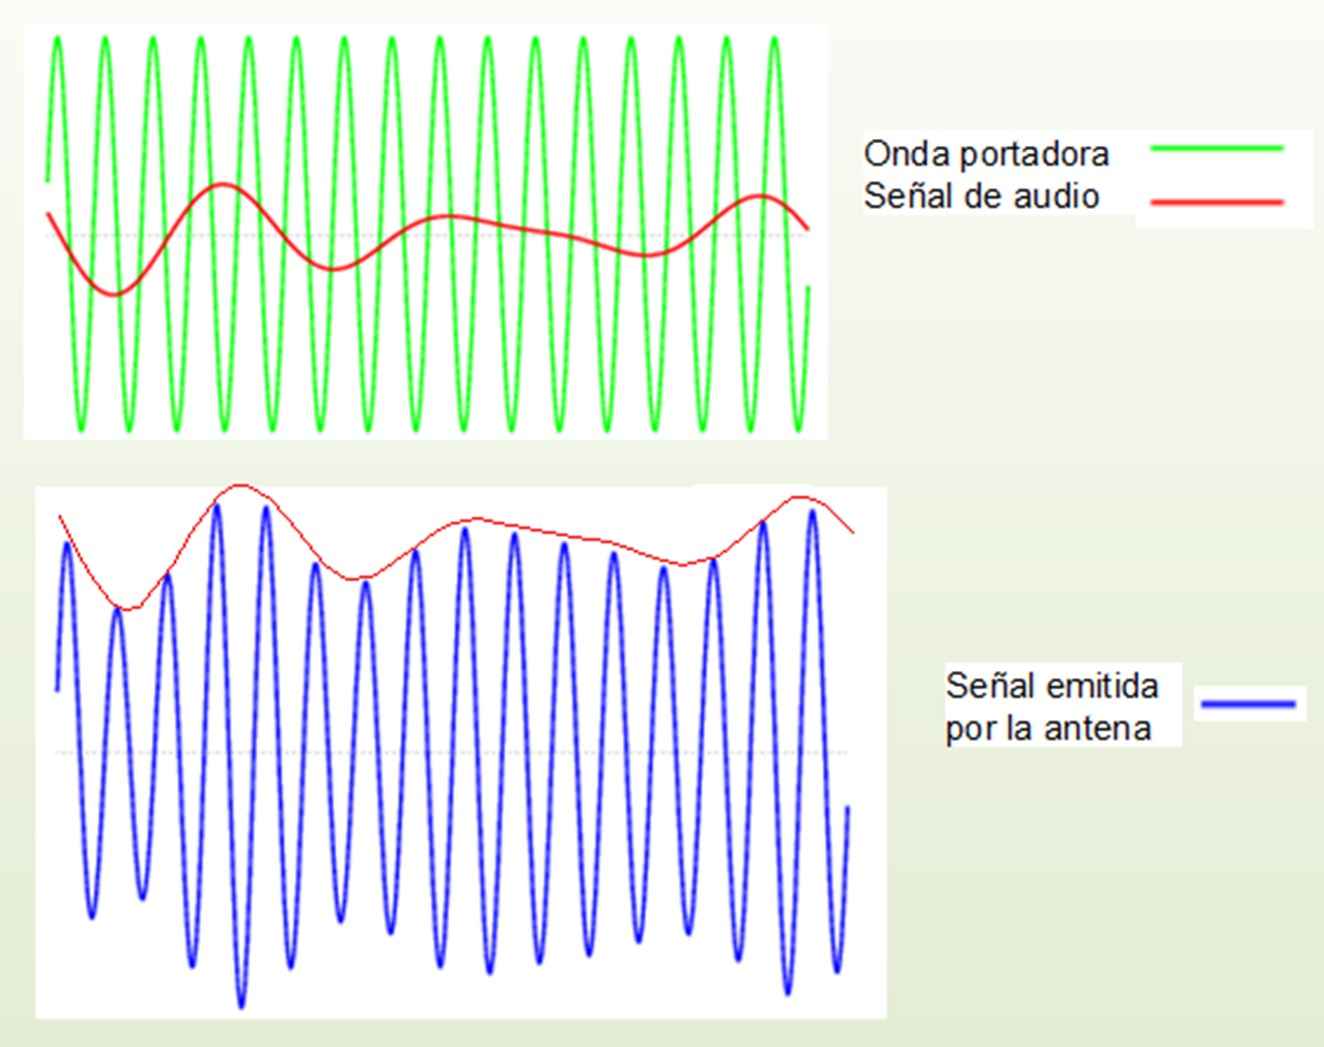
\includegraphics[scale=0.5]{Imagenes/am3.jpg}
	\label{fig:am_t}
    \captionsetup{justification=raggedright,font={scriptsize,bf,it}}
   \caption*{}
\end{figure}

\subsubsection{La Modulación de Frecuencia}
En la modulación de frecuencia (FM) el modelo anterior cambia de la siguiente manera:

\begin{equation} \label{equ_quince}
A(t)=A_c
\end{equation}

\begin{equation} \label{equ_dieciseis}
F(t)= K_f m(t)
\end{equation}

\begin{equation} \label{equ_diecisiete}
B(t)= 0
\end{equation}

Donde $K_f$ se conoce como coeficiente de modulación de frecuencia. Entonces se obtiene la señal modulada $s(t)$:

\begin{equation} \label{equ_diesiocho}
	s(t)=A_c cos[2 \pi (f_c+K_f m(t))t]
\end{equation}

Mediante algunas mejoras a la fórmula anterior se puede llegar a una expresión más conocida para la modulación FM.

\begin{equation} \label{equ_diesinueve}
s(t)=A_c cos[2 \pi f_c t + K_f \int m(t) dt]
\end{equation} 

De la expresión anterior se deduce que la Modulación FM representa también una forma de modulación de fase.

\textcolor{red}{[Falta: Oscar Reyes: gráfica en el dominio del tiempo, parámetros.]}


\subsubsection{La Modulación de Fase}
En la modulación de fase (PM) el modelo anterior cambia de la siguiente manera:

\begin{equation} \label{equ_veinte}
A(t)=A_c
\end{equation} 

\begin{equation} \label{equ_veintiuno}
F(t)= 0 
\end{equation} 

\begin{equation} \label{equ_veintidos}
B(t)= K_p m(t)
\end{equation} 

Donde $K_p$ se conoce como coeficiente de modulación de fase. Entonces se obtiene la señal modulada $s(t)$:

\begin{equation} \label{equ_veintitres}
s(t)=A_c cos[2 \pi (f_c t + K_p m(t))]
\end{equation} 

\textcolor{red}{[Falta: Oscar reyes: gráfica en el dominio del tiempo, parámetros.]}
\subsubsection{Análisis en el dominio de las frecuencias}
\textcolor{red}{[Falta: Oscar reyes: La idea es realizar una comparación entre todos los tipos de modulación en el dominio de las frecuencias. Pero si el profe Oscar tiene otra idea, tambien es aceptable, por ejemplo que ese análisis se haga por cada uno de los tipos de modulación por separado]}
% \OR para revisar desde la notación misma....

\section{Señales aleatorias}

\subsection{Planteamiento del problema}

Hasta el momento, se han visto señales teóricas o deterministicas que pueden ser presentadas por fórmulas matemáticas u otras maneras. En el mundo real las señales son casi siempre aleatorias y eso hace que los conceptos vistos anteriormente no se pueden aplicar de manera directa. Por ejemplo, si pretendemos usar el concepto estricto de la TF para observar, en el dominio de las frecuencias la voz de una persona, deberíamos esperar a que esa persona hable durante toda su vida antes de aplicarle la TF, pues esta, por definición analiza la señal en el tiempo que va desde $t = -\infty $ hasta $t = \infty $. Es claro que esto no es viable en la mayoría de las aplicaciones prácticas debido a la necesidad de resultados en tiempos más reales.\\

Del análisis anterior surge la pregunta: ¿Es posible usar herramientas de análisis como la Transformada de Fourier, los filtros, los sistemas LIT, etc, que han tenido su origen en señales determinísticas, para analizar señales del mundo real donde predomina más bien la aleatoriedad y el caos? ¿cómo hacerlo?. 

\subsection{Promedios de tiempo en señales reales}
La respuesta está en la necesidad de adaptar esos conceptos a dos posibles campos:
\begin{itemize}
    \item La Teoría de señales aleatorias. La idea consiste en que si bien las señales son aleatorias, varios parámetros pueden ser vistos como determinísticos, al menos dentro de ciertos límites. Por ejemplo la media de una señal, la desviación estándar, la potencia promedio, la distribución de la potencia promedio en el dominio de las frecuencias, los cuales se pueden calcular de manera aproximada al observar el comportamiento de la señal durante un tiempo tan corto o tan grande como tan pequeña o grande sea la exactitud deseada.
    \item La Teoría de procesos estocásticos. puede ser visto como una mayor generalización de la teoría se señales aleatorias, cuando la cuestión no se trata de analizar una sola señal sino un grupo de ellas. Por ejemplo, supongamos que hemos reunido las señales de voz de muchas personas diferentes para probar cómo se comportan al pasar por un sistema. El promedio de esas señales es otra señal que varía en el tiempo, pero que tiene un comportamiento más predecible.
\end{itemize}

En este capítulo solo hablaremos de la Teoría de señales aleatorias. Supongamos que en el problema en que usted trabaja solo se cuenta con una señal aleatoria, debido a las especificidades de ese problema. Es claro que esa señal tiene una media y por lo tanto todos esos parámetros que se derivan de la media, como la media cuadrática, la varianza, la desviación estándar, etc. Incluso la función de distribución de probabilidad. En este caso, el concepto que se usa se conoce como Promedios de Tiempo. Los cálculos son similares a los que se realizan con una Variable Aleatoria, la diferencia está esa variable tiene un resultado en cada instante de tiempo y que hay infinitos instantes de tiempo, ya que el tiempo es continuo. \\

El promedio de tiempo para una señal $a(t)$ se representa como $<a(t)>$ y se halla así.

\begin{equation} \label{equ_veinticuatro}
<a(t)> = \lim_{T \to \infty} \frac{1}{2T} \int_{-T}^{T} a(t)dt = \lim_{T \to \infty} \frac{1}{2T} \int_{-T}^{T} a_{T}(t)dt 
\end{equation} 

Donde $a_{T}(t)$ es una versión truncada de $a(t)$ como se muestra en la siguiente figura.

%\setcounter{figure}{29}
%\vspace{200px} 
\begin{figure}[h!]
	\captionsetup{justification = raggedright, singlelinecheck = false}
	\caption{Señal truncada} 
	\centering
	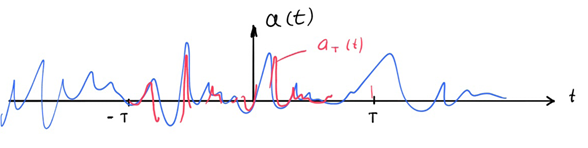
\includegraphics[scale=1]{Imagenes/Truncada.png}
	\label{fig:Truncada}
	%		\captionsetup{justification=raggedright,font={scriptsize,bf,it}}
	%		\caption*{fuente: http://superkuh.com/rtlsdr.html}
\end{figure}

Como puede observarse, entre más grande sea T, más alta es la exactitud en el cálculo del promedio de una señal.

\subsection{La Media de una Señal x(t)}

La Media De una señal x(t): La media De una señal x(t): 
 
 \begin{equation} \label{equ_veinticinco}
	 X_{m} = <x(t)> 
 \end{equation} 

\subsection{La Media Cuadrática de una Señal x(t)}
La Media Cuadrática De Una señal x(t): La media cuadrática de Una señal x(t):

 	\begin{equation} \label{equ_veintiseis}
		 X_{c} = <x^{2}(t)> 
	\end{equation}

\subsection{El Valor RMS}

El Valor RMS (del inglés Root Mean Square que se traduce como Raiz del Valor Medio Cuadrático)  de Una señal x(t): El Valor RMS de una Señal x(t):

	 \begin{equation} \label{equ_veintisiete}
	 	X_{RMS} = \sqrt{<x^{2}(t)>} 
	\end{equation}

\subsection{La Potencia Promedio de una Señal x(t)}

La Potencia Promedio Normalizada De Una señal

\begin{equation} \label{equ_veintiocho}
	 P = X_{RMS}^{2} = <x^{2}(t)> 
\end{equation} 


\textbf{Nota: el término “normalizada” es porque se considera $R=1 \Omega$}

\subsection{La Función de Autocorrelación}

La Función de Autocorrelación de x(t): La Función de Autocorrelación de x(t):

 \begin{equation} \label{equ_veintinueve}
	 R_{X}(\tau) = <x(t) x(t + \tau)> = \lim_{T \to \infty} \dfrac{1}{2T} \int_{-T}^{T} x(t) x(t + \tau) d\tau 
\end{equation}
Es importante notar que:
\begin{itemize}
    \item la Función de Autorrelación evaluada en $\tau =0$, es igual a la media cuadrática de la señal
    \item Por lo anterior, si la media de la señal es cero, entonces la Función de Autorrelación evaluada en $\tau =0$, es igual a la Potencia Promedio de la señal.
\end{itemize}    
\subsection{Otros promedios de tiempo}
La Varianza
\begin{equation} \label{equ_veintiocho}
	 {\sigma_x}^2= <[x(t)-X_m]^2>
\end{equation} 
La Desviación Estándar
\begin{equation} \label{equ_veintiocho}
	 \sigma_x= \sqrt{<[x(t)-X_m]^2>}
\end{equation} 

\subsection{Promedios de tiempo en señales complejas}
En el caso de las señales complejas es especial, ya que una señal es una especie de matrimonio entre una señal real y una imaginaria, de modo que es una pareja inseparable de señales. En este caso, es importante tener en cuenta lo siguiente:
\begin{itemize}
    \item una señal compleja, aunque es un apareamiento entre dos señales, puede ser vista como una sola cosa si se representa como un vector en el plano complejo, el cual puede variar diversos parámetros como su velocidad, su magnitud, su fase.
    \item hablar del promedio de tiempo en una señal compleja es hablar del comportamiento promedio del vector.\\
    \item El promedio de tiempo se puede definir como el valor complejo, donde la parte real y la imaginaria resultan de sacar el promedio de tiempo de la parte real de la señal y de la parte imaginaria respectivamente. Lo cual, se traduce en el punto del plano complejo donde hay mayor probabilidad de encontrar al vector.
    \item En el caso de la media cuadrática es un tanto diferente; en vez de la media cuadrática, lo que se usa es la magnitud cuadrática media del vector en el plano complejo. Pero igualmente resulta en un valor complejo, donde la parte real y la imaginaria resultan de sacar la media cuadrática de la parte real de la señal y de la parte imaginaria respectivamente. Lo cual, se traduce en la longitud al cuadrado que tiene mayor probabilidad de encontrarse el vector.
    \item La magnitud media, se deduce de lo dicho anteriormente, ya que es la raiz cuadrada del magnitud cuadrática media.
    \item En este caso, la Potencia Promedio de una señal es claramente el cuadrado de la magnitud media.
\end{itemize}

De acuerdo a las consideraciones anteriores, la media de una señal compleja aleatoria es un valor complejo y le corresponde esta fórmula:

 	\begin{equation} \label{equ_veintiseis}
		 X_{m} = <x_{r}(t)>+j<x_{i}(t)> 
	\end{equation}
Donde $x_{r}(t)$ y $x_{i}(t)$ corresponden a la parte real y a la imaginaria respectivamente de la señal analizada 

La Magnitud media cuadrática de una señal compleja aleatoria es un valor real y le corresponde la siguiente fórmula:

 	\begin{equation} \label{equ_veintiseis}
		 |X_{c}| = <|x(t)|^{2}> 
	\end{equation}

También es válido decir que:
 	\begin{equation} \label{equ_veintiseis}
		 |X_{c}| = X_{rc}+X_{ic} 
	\end{equation}
Donde $X_{rc}$ y $X_{ic}$ son la media cuadrática de la parte real y de la parte imaginaria respectivamente de la señal analizada $x(t)$
A la Función de Autocorrelación le corresponde la fórmula:

 \begin{equation} \label{equ_veintinueve}
	 R_{X}(\tau) = <|x(t) x(t + \tau)|> = \lim_{T \to \infty} \dfrac{1}{2T} \int_{-T}^{T} |x(t) x(t + \tau)| d\tau 
\end{equation}

Potencia promedio normalizada es:
 	\begin{equation} \label{equ_veintiseis}
		 P=X_{c} 
	\end{equation}
De igual manera, se puede deducir que el Valor RMS para las señales complejas es:

	 \begin{equation} \label{equ_veintisiete}
	 	X_{RMS} = \srqt{|X_{c}|} = \sqrt{<|x(t)^{2}>}=\srqt{<|x(t)|>} 
	\end{equation}

	 \begin{equation} \label{equ_veintiocho}
	 	X_{RMS} = \sqrt{|X_c|} + \sqrt{|x(t)|^{2}>} + <|x(t)|>
	\end{equation}

\subsection{La Densidad Espectral de Potencia}



La PSD como un promedio de tiempo: Ya se ha dicho que la PSD es la distribución de la potencia promedio, de la señal analizada en el espectro de frecuencias. La PSD de una señal $x(t)$ se representa como $S_{X}(f)$. \\

Debido a la anterior afirmación se obtiene que:\\ 

\begin{equation} \label{equ_treinta}
	P =  \int_{-\infty}^{\infty} S_{X}(f) df 
\end{equation}

Aprovechando la relación de Parseval podemos encontrar dos maneras alternativas para hallar la Potencia Promedio de una señal $x(t)$:

\begin{equation} \label{equ_treintauno}
	 P = \lim_{T \to \infty} \dfrac{1}{2T} \int_{-\infty}^{\infty} |X_{T}(t)|^{2}dt  ;  P = \lim_{T \to \infty} \dfrac{1}{2T} \int_{-\infty}^{\infty} |X(f , T)|^{2}df 
\end{equation}

Donde $X(f,T)$ es la TF de $x_{T}(t)$ , luego: \\

\begin{equation} \label{equ_treintados}
X(f,T) = \int_{-\infty}^{\infty} x_{T}(t)e^{-j2\pi ft} dt = \int_{-T}^{T} x/(t)e^{-j2\pi ft} dt 
\end{equation}

Se deduce entonces que:

\begin{equation} \label{equ_treintatres}
	 S_{X}(f) = \lim_{T \to \infty} \frac{1}{2T} |X(f, T)|^{2} 
\end{equation}

Como es bien sabido, las dimensiones de la TF son en V/Hz, de modo que las de la TF en magnitud al cuadrado son en $Watts/Hz^{2}$. Por lo tanto, las de la PSD son de $watts/Hz$. Nota: se están considerando valores normalizados para $R = 1\Omega$ . Esto es útil cuando solo se desea conocer la forma del espectro, sin embargo, para mediciones más precisas de espectro, por ejemplo cuando se desea conocer el espectro que captura la antena de un USRP, hay que tener en cuenta que R es la impedancia del medio donde se mide la señal. El problema es que la impedancia de una antena es diferente para cada frecuencia.\\
\subsection{Relación de la Densidad Espectral de Potencia con la Función de Autocorrelación}
Existe una importante relación entre PSD y autocorrelación de una señal aleatoria la cual se expresa de la siguiente manera:
$S_{X}(f)$ es también la TF de $R_{X}(\tau)$ entonces, $S_{X}(f)=\int_{-\infty}^{\infty} R_{X}(\tau)e^{-j2\pi f\tau} d\tau$. Consecuentemente la potencia promedio se puede hallar también como $P=R_{X}(0)$.\\

\subsection{Periodograma}

Es la Gráfica que corresponde a la expresión $\dfrac{1}{2T}|X(f,T)|^{2}$ cuando se obtiene con elementos de cómputo. \\

En este caso resulta más útil la formulación

\begin{equation} \label{equ_treintacuatro}
  S_{x}(f) = \lim_{T \to \infty} \dfrac{1}{2T} |X(f,T)|^{2} = <|X(f)|^{2}> 
\end{equation}

La idea es caer en cuenta que esta fórmula expresa un promedio. En simulink o en GNU Radio se puede ir mostrando cómo se va calculando ese promedio a medida que pasa el tiempo. De modo que no es necesario esperar a que transcurra todo el tiempo T para visualizar la PSD. \\

%\vspace{200px}
\begin{figure}[h!]
	\captionsetup{justification = raggedright, singlelinecheck = false}
	\caption{Ejemplo de periodograma} 
	\centering
	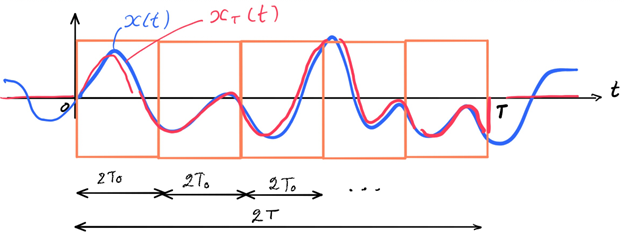
\includegraphics[scale=0.8]{Imagenes/Periodograma.png}
	\label{fig:Ejemplo-periodo}
	%		\captionsetup{justification=raggedright,font={scriptsize,bf,it}}
	%		\caption*{fuente: http://superkuh.com/rtlsdr.html}
\end{figure}

La idea es dividir el tiempo de medición T en pequeñas ventanas de duración $T_{0}$. Entonces la señal truncada $X_{T}(t)$ se divide en señales sub truncadas de más corta duración $ x_{T,1}(t), x_{T,2}(t), .... , x_{T,N}(t) $ De esta manera, es posible hallar paso a paso $ |X_{1}(f,T)|^{2}, |X_{2}(f,T)|^{2}, .... , |X_{N}(f,T)|^{2} $ consecuentemente se puede hallar la PSD aproximada de esas señales sub truncadas $ S _{X,1}(f,T), S _{X,2}(f,T).... S _{X,N}(f,T)$. Si en cada uno de esos pasos se va realizando un ajuste, será posible obtener y graficar la PSD para el tiempo $ 2T_{0}, 4T_{0}, 6T_{0}, ..... , 2T$. . Como resultado veremos como la PSD va tomando poco a poco una forma cada vez más definida. Lo que se logra es que el usuario no tenga que esperar mucho tiempo para ver la PSD, sino que en tiempo real pueda ver como la PSD va tomando una forma cada vez más definitiva. Para el ajuste mencionado solo hay que tener en cuenta que la PSD es un promedio, pero eso se explicará más abajo en una implementación que usa la FFT como bloque de cálculo de la Transformada de Fourier Truncada. \\

Uso del bloque FFT de GNU Radio para obtener la PSD. La idea es usar el bloque de GNU Radio que implementa el algoritmo FFT en magnitud al cuadrado, que simbolizaremos así:
$|FFT|^{2}$. En la página web del libro, se tiene una demostración donde se usa Simulink de Matlab para demostrar lo anterior, este es el enlace:

\begin{center}
\url{https://sites.google.com/saber.uis.edu.co/comdig/m/Analizador}
\end{center}

\subsection{Señal Binaria Bipolar Aleatoria}
Uno de los primeros pasos en el estudio de las comunicaciones consiste en conocer y analizar ciertas señales que son claves. Una de ellas son las señales binarias bipolares aleatorias.\\ 
Obtenemos primero La función de autocorrelación. Tomaremos como ejemplo la señal $x(t)$. de la Figura \ref{fig:Ejemplo} donde $T_b$ es el ancho de cada pulso que en términos de señales digitales, puede ser equivalente a la duración de un bit.

\begin{figure}[h!]
	\captionsetup{justification = raggedright, singlelinecheck = false}
	\caption{Ejemplo de una señal binaria aleatoria bipolar $x(t)$ } 
	\centering
	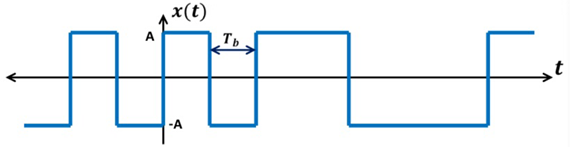
\includegraphics[scale=0.9]{Imagenes/Ejemplo.png}
	\label{fig:Ejemplo}
	%		\captionsetup{justification=raggedright,font={scriptsize,bf,it}}
	%		\caption*{fuente: http://superkuh.com/rtlsdr.html}
\end{figure}

Recordemos que $ R_{X}(\tau) = <x(t)x(t + \tau)> = \lim_{T \to \infty} \dfrac{1}{2T} \int_{-T}^{T} x(t) x(t + \tau ) d\tau $. En la Figura \ref{fig:Ejemplo1} set tiene la forma de la señal $x(t+\tau)$ cuando $\tau<T_b$\\

\begin{figure}[h!]
	\captionsetup{justification = raggedright, singlelinecheck = false}
	\caption{El desplazamiento de la señal binaria aleatoria bipolar que resulta en la señal $\tau < T_b $} 
	\centering
	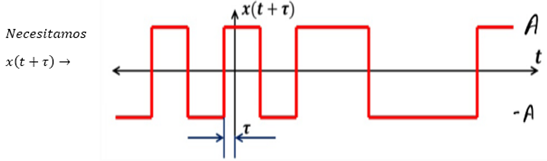
\includegraphics[scale=1]{Imagenes/Ejemplo1.png}
	\label{fig:Ejemplo1}
	%		\captionsetup{justification=raggedright,font={scriptsize,bf,it}}
	%		\caption*{fuente: http://superkuh.com/rtlsdr.html}
\end{figure}
Vamos a revisar los siguientes casos:
\begin{itemize}
    \item Caso en que $\tau = 0$:\\
Tenemos que $<x(t) x(t + \tau )> =<x^{2}(t)>=<A^{2}>=A^{2}$
    \item Caso en que $0<\tau<T_b$:\\
En este caso, la operación $x(t)x(t+\tau)$ tiene la forma que se presenta en la Figura \ref{fig:Ejemplo2}.
\begin{figure}[h!]
	\captionsetup{justification = raggedright, singlelinecheck = false}
	\caption{Multiplicación de la señal $x(t)$ con su versión desplazada $x(t+\tau)$ cuando $0<\tau < T_b$}
	\centering
	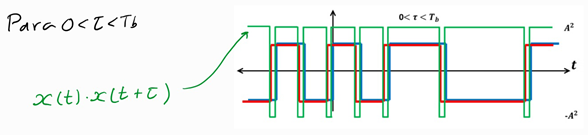
\includegraphics[scale=1]{Imagenes/Ejemplo2.png}
	\label{fig:Ejemplo2}
	%		\captionsetup{justification=raggedright,font={scriptsize,bf,it}}
	%		\caption*{fuente: http://superkuh.com/rtlsdr.html}
\end{figure}
    \item Caso en que  $ \tau = T_{b}$:
Tenemos que la multiplicación $x(t)x(t+\tau)$ resulta siendo una nueva señal binaria aleatoria bipolar como se muestra en la Figura \ref{fig:Ejemplo3}.
\begin{figure}[h!]
	\captionsetup{justification = raggedright, singlelinecheck = false}
	\caption{Multiplicación de la señal $x(t)$ con su versión desplazada $x(t+\tau)$ cuando $0<\tau = T_b$}
	\centering
	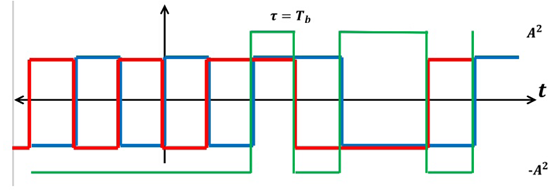
\includegraphics[scale=0.9]{Imagenes/Ejemplo3.png}
	\label{fig:Ejemplo3}
	%		\captionsetup{justification=raggedright,font={scriptsize,bf,it}}
	%		\caption*{fuente: http://superkuh.com/rtlsdr.html}
\end{figure}
\end{itemize}

Vemos que para $ \tau = 0, x(t)x(t + \tau ) = A^{2}$ y su promedio de tiempo es $<x(t)x(t+\tau ) > A^{2}$ que es la misma potencia promedio. Cuando $0 < \tau < T_{b}$ el promedio de tiempo de $x(t)x(t+\tau)$ cae linealmente.
Cuando $ \tau = T_{b}$  ocurre que $x(t)x(t + \tau)$ se convierte en una nueva señal binaria bipolar aleatoria, cuyo promedio de tiempo es cero. Algo similar ocurre cuando $\tau > T_{b}$.
Ahora, cuando $\tau < 0$ ocurre lo mismo que cuando $\tau > 0$.


Es importante tener en cuenta que la Función de Autocorrelación evaluada en cero es la misma potencia promedio $P=R_{X}(0)$, solo que para el caso dado, $P=R_{X}(0)=A^2$. De modo que la función de autocorrelación tiene la forma de la Figura \ref{fig:Triangulo}.

%\vspace{200px}
\begin{figure}[h!]
	\captionsetup{justification = raggedright, singlelinecheck = false}
	\caption{La Función de Autocorrelación de una señal binaria aleatoria bipolar} 
	\centering
	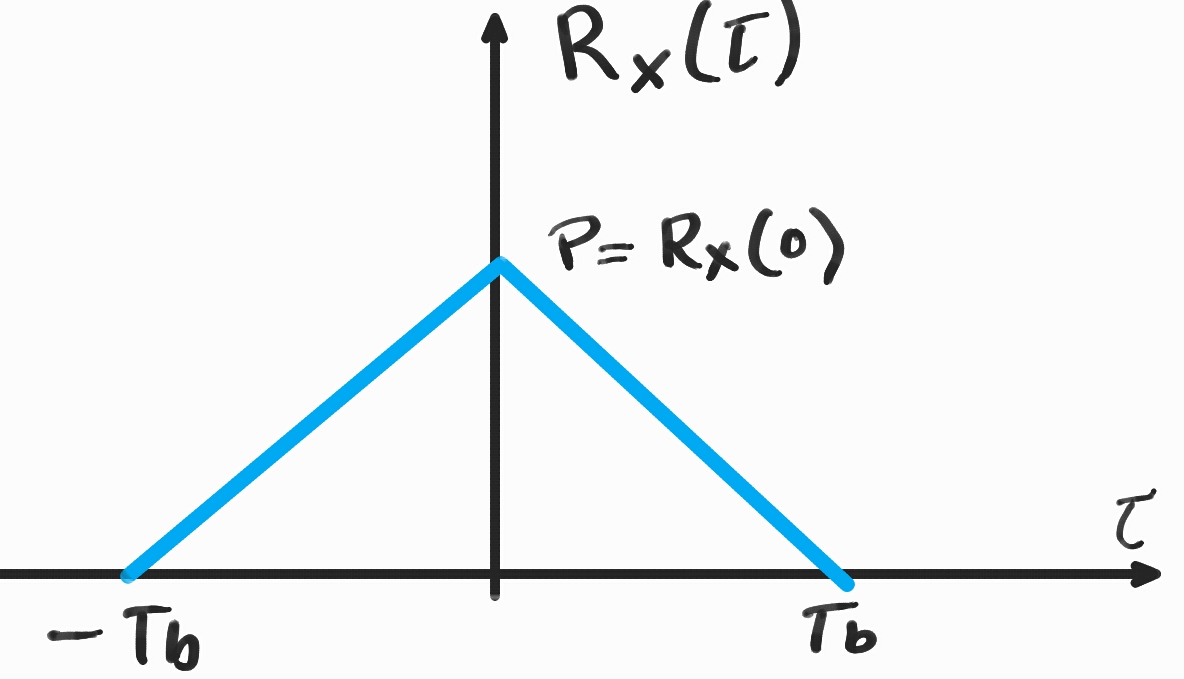
\includegraphics[scale=0.3]{Imagenes/Triangulo.png}
	\label{fig:Triangulo}
	%		\captionsetup{justification=raggedright,font={scriptsize,bf,it}}
	%		\caption*{fuente: http://superkuh.com/rtlsdr.html}
\end{figure}

Recordemos que la PSD es la TF de la Función de Autocorrelación. De manera que podemos usar la Función de Autocorrelación obtenida para buscar la forma de la PSD. Para ello, expresamoos la Función de autocorrelación como una Convolución así:

\begin{equation} \label{equ_treintacinco}
	 R_{x}(\tau) =\frac{1}{T_{b}} R_{X1}(\tau) * R_{X1}(\tau) 
\end{equation}

Donde $R_{X1}(\tau)$ tiene una forma rectangular como se muestra en la siguiente figura \ref{fig:Cuadrado}.



\begin{figure}[h!]
	\captionsetup{justification = raggedright, singlelinecheck = false}
	\caption{ Forma de $R_{X1}(\tau)$} 
	\centering
	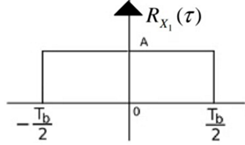
\includegraphics[scale=1]{Imagenes/Cuadrado.png}
	\label{fig:Cuadrado}
	%		\captionsetup{justification=raggedright,font={scriptsize,bf,it}}
	%		\caption*{fuente: http://superkuh.com/rtlsdr.html}
\end{figure}

De esta manera podemos usar la TF de una señal de forma rectangular, la cual es bien conocida y que se muestra en la Figura \ref{fig:Cuadrado-dos}.

\begin{figure}[h!]
	\captionsetup{justification = raggedright, singlelinecheck = false}
	\caption{$R_{X_1}(\tau)$ y su Transformada de Fourier} 
	\centering
	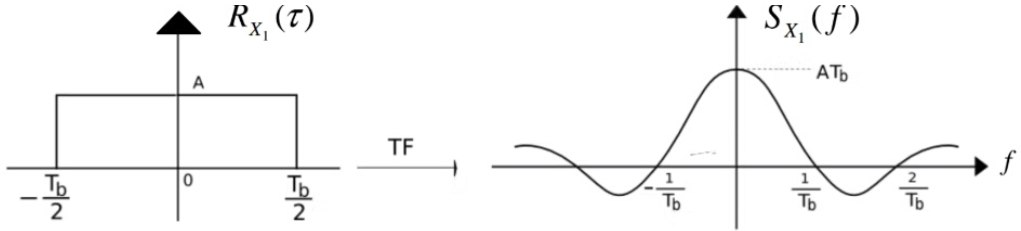
\includegraphics[scale=0.6]{Imagenes/Cuadrado-dos.png}
	\label{fig:Cuadrado-dos}
	\captionsetup{justification=raggedright,font={scriptsize,bf,it}}
\end{figure}

Nótese que $S_{X_1}(f)$ estaría dado en V/Hz tal como se conoce la TF de una señal cuadrada. \\
También aprovechamos el Teorema de la Convolución, también conocido como Teorema de Wiener Khitchine que dice que si se tiene:

\begin{equation} \label{equ_treintaseis}
	x_{1}(t) = \overset{TF}{\rightarrow} X_{1}(f) 
\end{equation}
y
\begin{equation} \label{equ_treintasietex}
	x_{2}(t) = \overset{TF}{\rightarrow} X_{2}(f)
\end{equation}

Entonces
\begin{equation} \label{equ_treintasiete}
	 x_{1}(t) * x_{2}(t) \overset{TF}{\rightarrow} X_{1}(f) X_{2}(f)
\end{equation}

Luego,

\begin{equation} \label{equ_treintaocho}
\frac{1}{T_b}R_{X_1}(\tau )*R_{X_1}(\tau )\overset{TF}{\rightarrow}\frac{1}{T_b}S^{2}_{X_{1}}(f)
\end{equation}

\begin{figure}[h!]
	\captionsetup{justification = raggedright, singlelinecheck = false}
	\caption{ PSD de la forma Forma de $R_{X1}(\tau)$} 
	\centering
	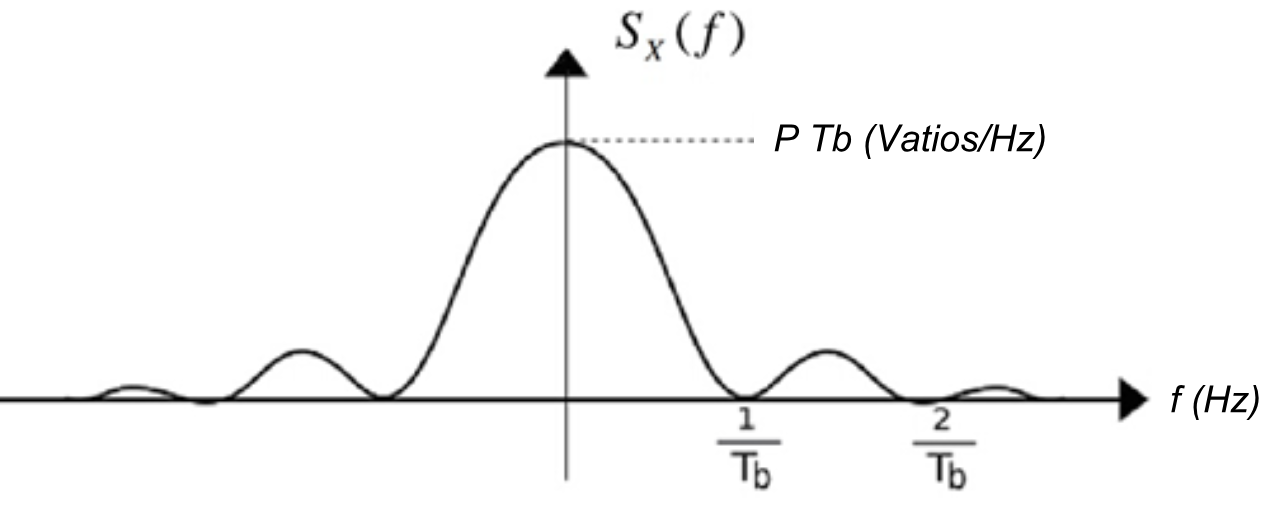
\includegraphics[scale=0.4]{Imagenes/PSD.png}
	\label{fig:PSD}
	%		\captionsetup{justification=raggedright,font={scriptsize,bf,it}}
	%		\caption*{fuente: http://superkuh.com/rtlsdr.html}
\end{figure}
De esta manera se obtiene que la forma de la PSD de una señal binaria aleatoria bipolar corresponde a la función sinc cuadrática:
\begin{equation} \label{equ_treintasietess}
	 S_X(f)=P T_b sinc^2(f/R_b)
\end{equation}
donde $R_b=1/Tb$ es la rata de bits. La gráfica de la PSD de una Función Binaria Aleatoria Bipolar se presenta en la Figura \ref{fig:PSD}.

\subsection{El ruido blanco}

El ruido blanco (WN, del inglés White Noise) siempre está presente en cualquier medio de propagación, pero no deja de ser una abstracción matemática, debido a ciertos supuestos como: 

\begin{itemize}
	
	\item  Tienen un ancho de banda infinito. De allí viene el término “blanco”, pues se supone que el color blanco resulta de combinar homogéneamente todos los colores (las frecuencias).
	\item  La Densidad Espectral de Potencia es constante e igual a $N_0/2$, donde 

\begin{equation} \label{equ_treintanueve}
		 N_0 = kT_e
\end{equation}

Donde $k$ es la constante de Boltzmann y $T_e$ es la temperatura equivalente del ruido en el receptor. La idea de la temperatura equivalente proviene de experimentos realizados con sistemas electrónicos, donde se ha observado a que a medida que aumenta la temperatura en estos sistemas, aumenta el ruido. En gran manera puede estar dado por las características del receptor, pero también por cuestiones naturales en el espectro.

	\item  La función de autocorrelación es una función delta centrada en cero, como se muestra en la Figura \ref{fig:Funcion}, lo cual significa que dos muestras del ruido, por muy cercanas que sean no están correlacionadas, de modo que una muestra aparece correlacionada solo con sí misma. En este sentido, el ruido blando es lo último en aleatoriedad.
	
%	\setcounter{figure}{47}
	\begin{figure}[h!]
		\captionsetup{justification = raggedright, singlelinecheck = false}
		\caption {PSD del ruido blanco y su Función de autocorrelación} 
		\centering
		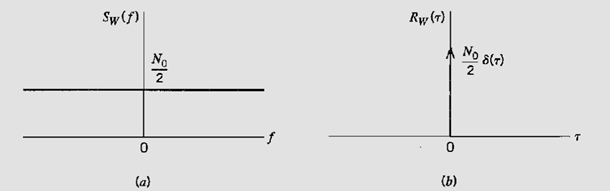
\includegraphics[scale=0.9]{Imagenes/Funcion.png}
		\label{fig:Funcion}
				\captionsetup{justification=raggedright,font={scriptsize,bf,it}}
				\caption*{fuente: Tomado del libro de Haykin}
	\end{figure}
	\item  Conocer el desempeño de un sistema de comunicaciones frente al ruido blanco que puede presentarse en el canal, no deja de ser una idealización, pero sirve de referencia para caracterizar el sistema y los métodos usados en el procesamiento de la información.  
\end{itemize}


\subsection{La voz humana} en la telefonía

El sonido es uno de los principales tipos de mensajes que se emiten por los medios de comunicación y se usa intensamente en ejemplos y prácticas de este libro, sobre todo los sonidos que el ser humano emite para comunicar. La voz es toda una ciencia, sinembargo, para los propósitos del presente libro los siguientes apuntes son los de mayor relevancia:
\begin{itemize}
    \item el sonido son ondas mecánicas longituinales, se desplazan de un lugar a otro mediante perturbaciones de un medio elástico (sólido, líquido, gaseoso).
    \item Las ondas sonoras se reducen a los límites de frecuencia que pueden estimular el oido humano para ser percibidas en el cerebro.
    \item los límites de frecuencia de las ondas sonoras se extienden de aproximadamente 20 Hz a cerca de 20 kHz y se llaman límites de audición.
    \item La voz está constituida por un conjunto de sonidos generados por el aparato fonador, de manera que tiene un menor rango de frecuencias que el sonido
    \item En aplicaciones reales de comunicaciones, una señal de voz es una señal aleatoria, desde este punto de vista sus características son de tipo aleatorio, pero además depende de cada persona.
    \item De acuerdo a los estudios tenidos en cuenta por la UIT, la mayor energía de la voz se encuentra concentrada por debajo de los 4 kHz. De modo que la UIT ha establecido que para los propósitos de la telefonía, la señal de la voz puede estar limitada a 4 kHz. Es por eso que, al implementarse las tecnologías digitales en la frecuencia fija, se estableció que la frecuencia de muestreo es de $Samp rate   audio=8$  kHz. También se estableció que los niveles de cuantificación son 256, lo cual equivale a 8 bits por muestra ya que $NbpS=256=2^8 $ 
    \item De lo anterior se deduce que la rata de bits en la telefonía es de $Rb=Samp rate audio x Nbps=64$ kbps.
\end{itemize}

\section{Variable aleatoria.}
\subsection{Introducción}
Arriesgarse a estudiar y sobre todo a practicar con señales aleatorias  significa arriesgarse a contactar con el mundo real. Esto es así, pues en el mundo real las señales son usualmente aleatorias. Pero surge una pregunta: ¿No basta con haber estudiado el tema de promedios de tiempo para realizar aplicaciones basadas Radio Definida por Software (SDR)? La respuesta es que sí. Sin embargo, estudiar el tema de Variable Aleatoria significa una especie de reconciliación con los matemáticos que trabajan en función de aplicaciones más amplias, que muchas veces no tienen que ver con señales, pero que pueden ser adaptadas a las señales y a los sistemas.\\ 
A manera de ejemplo, imaginemos que contamos con una señal de ruido discreta $x[n]$ de $N$ muestras y que hemos convocado a diferentes expertos a hablar sobre ella y a realizar demostraciones. Nosotros, realizaríamos quizá una simulación con gnuradio para mostrar cómo esta señal $x[n]$ esa compuesta de las muestras $x[1], x[2], ..., x[N]$ que tienen un comportamiento en tiempo y en frecuencia. También podríamos mostrar promedios de tiempo de esa señal, como la media, la varianza, etc. 
El siguiente experto podría ser un matemático o un ingeniero de sistemas que es muy hábil usando las herramientas que traen muchos lenguajes de programación para realizar operaciones vectoriales y matriciales que agilizan de manera severa el desarrollo de código. Entonces prefiere ver esa señal como un vector $\Vec{X}=[x_1, x_2, ...., x_{N}]$ al cual podrá manejar mediante operaciones vectoriales o matriciales. 
Supongamos que el experto es ahora un profesor de estadística acostumbrado a estudiar el comportamiento de ciertas variables como el precio del dolar, la frecuencia de las lluvias, etc. Este profesor prefería ver la  señal como un dataset o conjunto de los datos de las amplitudes que puede tomar la señal para obtener diversos parámetros y conceptos estadísticos como: la media, la varianza, pero también la función de densidad de probabilidad, la función de distribución acumulativa, la autocorrelación, entre otros. En este caso, la variable aleatoria y los promedios de tiempo son una misma cosa. Pero una variable aleatoria es un concepto más general pues abarca muchos otros casos, donde los datos que toma la variable no dependen necesariamente del tiempo. Por ejemplo, supongamos que la variable aleatoria $Z$ está compuesta de los N valores que resultan al lanzar un dado N veces. Esos N resultados no dependen del tiempo ni tienen nada que ver con las amplitudes de las señales.\\ 
En conclusión, lo que se gana al usar el concepto de Variable Aleatoria es la posibilidad de aprovechar en las comunicaciones los avances que existen en la estadística. La podemos usar como una alternativa a los promedios de tiempo. Para ello basta con suponer que cada muestra de la señal es el resultado de un ensayo. Pero el concepto de variable aleatoria se puede usar en un sentido más amplio donde los parámetros a analizar no son necesariamente valores de amplitud que cambian en el tiempo. En todo caso, el estudio del tema de Variable Aleatoria es imprescindible para llegar a estudiar el tema de Procesos Estocásticos que es una rama más genérica aún para estudiar las señales aleatorias en un sentido más amplio, por ejemplo, cuando nos interesa conocer el promedio de las voces de todos mis estudiantes, lo cual resulta en una nueva señal de tiempo que es el promedio de todas\\

Para aclarar aún más el concepto de variable aleatoria, supongamos que usted ha sido contratado para  para caracterizar la estatura de los estudiantes de su universidad. Entonces usted decide usar los siguientes parámetros: la estatura promedio, la desviación estándar, entre otros. Luego, usted decide realizar un experimento: medir de manera aleatoria a cada estudiante que entra ese día a la universidad. También querrá medir de manera aleatoria otras cosas que pueden guardar relación obvia o no tan obvia con la estatura como: la edad o el número de calzado, el sexo. Entonces crea una tabla con una columna para cada una de las mediciones, donde X representa la estatura, Y la edad y Z el calzado. X, Y, Z - son variables aleatorias. \\
En conclusión, el concepto de variable aleatoria es útil en las comunicaciones, cuando se desea interpretar las caracterísiticas de las señales o de los sistemas como datos para aplicarle conceptos estadísticos para llegar a algún tipo de conclusión válida.


\begin{table}[h!]
	\captionsetup{justification = raggedright,singlelinecheck = false}
	\caption{\label{tabla:tabla1} Alguna descripción}
		\centering
		\scalebox{0.75}{
\begin{tabular}{|l|l|l|l|}
\hline
Ensayo & X   & Y   & Z   \\ \hline
1      & $x_{1} = 1.80$   & $y_{1} = 18$   &  $z_{1} = 40$   \\ \hline
2      & $x_{2} = 1.70$   & $y_{2} = 20$   &  $z_{2} = 39$   \\ \hline
3      & $x_{3} = 1.73$   & $y_{3} = 17$   &  $z_{3} = 43$  \\ \hline
...    & ... & ... & ... \\ \hline
\end{tabular}}
\end{table}

También puede usar la siguiente notación: \\
$X= {x_{1}, x, x,...}$ \\

\subsection{Principales conceptos de variable aleatoria}

Los siguientes son los principales términos usados: \\

\textbf{Ensayo (realization):} Cada prueba que usted realiza. \\

\textbf{ Punto Muestra o Punto Muestral (sample point):} El resultado de cada ensayo, en este caso xi es el punto muestral del ensayo i de la variable aleatoria X. \\

\textbf{ Espacio muestral (Sample Space):} Es el conjunto de todos los puntos muestra posible para variable aleatoria. \\

\textbf{ La Esperanza (average or expected value):} Es la manera de referirse al promedio de puntos muestra y se representa como E[variable aleatoria] así: \\


\begin{equation} \label{capuno_variable}	
E[X]= \dfrac{x_{1} + x_{2} + ... + x_{N} }{N} ; E[X^{2}]= \dfrac{x_{1}^{2} + x_{2}^{2} + ... + x_{N}^{2} }{N}
\end{equation}

\begin{equation} \label{capuno_variabledos}	
E[({X-A})^{2}]=  \dfrac{{(x_{1}-A)}^{2} + {(x_{2}-A)}^{2} + ... + {(x_{N}-A)}^{2} }{N}
\end{equation}

$N$ Es el número de puntos muestra tenidos en cuenta. \\
Pero hay casos en que no se conocen los puntos muestra sino otros parámetros que se han obtenido a partir de ellos y que también definen la variable aleatoria como la Función de Densidad de Probabilidad $f_{X}(x)$. Por eso hay otras formas para obtener la Esperanza como $E[X]=-\int_{\infty}^{\infty}xf_{X}(x)dx$. \\

\textbf{ La media de una variable aleatoria} $X: \mu X=E[X]$ \\
\textbf{ La media cuadrática de una variable aleatoria} X: Corresponde a $E[X^{2}]$ \\
\textbf{ La varianza de una variable aleatoria} $X: var[X]=E[{(X- \mu X)}^{2}]= {\sigma}_{X}^{2}$ \\
\textbf{ La Desviación estándar de} $ X :$ es ${\sigma}_{X}$\\
\textbf{ La correlación entre las variables} $ X,Y: R_{XY}=E[XY]$\\

\subsection{La Función de densidad de probabilidad}
La Función de Densidad de Probabilidad (FDP) describe la probabilidad que puede cada valor que puede tomar una variable aleatoria. También permite conocer la probabilidad de que una variable aleatoria caiga dentro de un rango de posibles valores. Para los propósitos de este resumen, resulta suficiente comprender lo que representa la curva de la FDP en un ejemplo como el que se presenta en la en la figura \ref{fig:fdp}. 


\begin{figure}[h!]
	\captionsetup{justification = raggedright, singlelinecheck = false}
	\caption{Ejemplo de la Función de Densidad de probabilidad} 
	\centering
	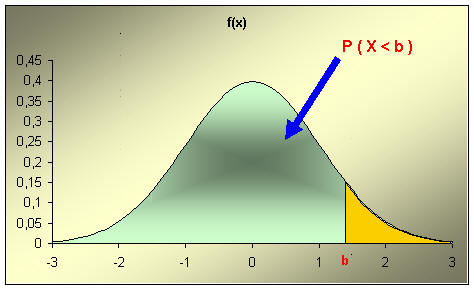
\includegraphics[scale=0.5]{Imagenes/probcon3.jpg}
	\label{fig:fdp}
% Lo siguiene es para indicar la fuente de la cual fue tomada la figura
  \captionsetup{justification=raggedright,font={scriptsize,bf,it}}
\end{figure}

Para el ejemplo que representa esa figura, podemos observar que la probabilidad de que la variable aleatoria $X$ tome el valor 1 es aproximadamente 0,15, que si se expresa en porcentaje, equivale al 15\%. El área bajo la curva de la FDP es siempre igual a 1. La probabilidad de que la variable aleatoria tome un valor menor que b, es decir $P(X<b)$ es igual al área bajo la curva desde $-\infty$ hasta b y para el ejemplo dado en la figura \ref{fig:fdp} se encuentra sombreada en color azul. De manera similar, buscando siempre el área bajo la curva entre intervalos diversos es posible encontrar la probabilidad de que $X$ tome cualquier otro rango de valores.\\

Un aspecto muy importante a tener siempre en cuenta es que al FDP caracteriza completamente a una variable aleatoria. Es decir, si se conoce la FDP de una variable aleatoria, ya se tiene toda la información sobre esa variable.


En gnuradio es común aproximarse a la FDP mediante lo que se conoce como un histograma, mientras que el uso de una forma continua de la FDP es más común en los análisis teóricos. En los histogramas usualmente se considera que la variable aleatoria puede tomar un número finito de valores discretos, como se muestra en el ejemplo de la figura \ref{fig:histo}. 

\begin{figure}[h!]
	\captionsetup{justification = raggedright, singlelinecheck = false}
	\caption{Ejemplo de un histograma} 
	\centering
	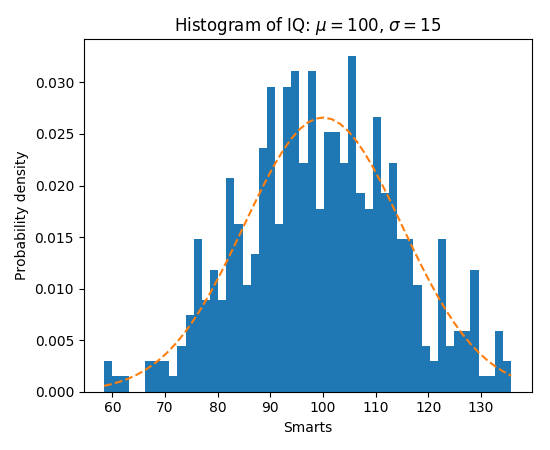
\includegraphics[scale=0.5]{Imagenes/histogram_demo_features.png}
	\label{fig:histo}
% Lo siguiene es para indicar la fuente de la cual fue tomada la figura
  \captionsetup{justification=raggedright,font={scriptsize,bf,it}}
  \caption*{fuente: Matplolib}
\end{figure}

\subsection{La Función de Distribución Acumulativa}
La Función de Distribución Acumulativa (FDA) es otra manera de caracterizar completamente una variable aleatoria, pero no es nada nuevo con respecto a la FDA, sino más bien una deducción de ella, ya que la FDA se puede expresar como

\begin{equation} \label{equ:fda}
	 F(x)=\int\limits_{-\infty}^{x}  f(u)du,				
\end{equation}
donde $f(u)$ es la FDP de una variable aleatoria $U$.

\section{Procesos Estocásticos}

Los procesos estocásticos representan un mayor nivel de generalización de las variables aleatorias para poner la teoría de las probabilidades al servicio exclusivo de las señales aleatorias. En este sentido, es importante tener en cuenta las siguientes aclaraciones:
\begin{itemize}
    \item Una variable aleatoria toma valores que dependen de un ensayo. Por ejemplo, si el experimento consiste en medir la altura de los estudiantes, cada estudiante que medimos es un ensayo y la altura de medimos es una muestra de la variable aleatoria.
    \item Es posible hacer que una variable aleatoria tome como muestras los valores de amplitud que toma una señal en el tiempo, pero precisamente eso es un caso muy particular que hemos llamado Promedios de Tiempo. En los procesos estocásticos no se tiene esta posibilidad, ya que en un proceso estocástico una señal en el tiempo considerado como el resultado de un ensayo, por eso se habla de funciones muestra.
\end{itemize}

Para entenderlo mejor, supongamos que hemos sido contratados para caracterizar no la altura, sino la voz de los estudiantes de su universidad. Entonces, en lugar de medir la altura para llenar una lista de datos, lo que hacemos es grabar la voz de cada estudiante que pasa aleatoriamente y la guardamos. Entonces, ya no tenemos muestras discretas en forma de un valor por muestra, como era el caso para la altura, sino funciones funciones muestra, ya que cada muestra es una función de tiempo, como se muestra en la figura \ref{fig:Ensayo}.

	\begin{figure}[h!]
		\captionsetup{justification = raggedright, singlelinecheck = false}
		\caption{Ejemplo de Funciones muestra de un proceso estocástico $X(t)$} 
		\centering
		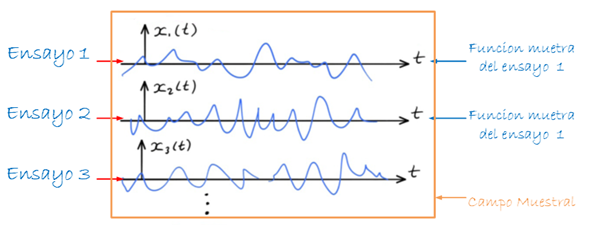
\includegraphics[scale=1]{Imagenes/Ensayo.png}
		\label{fig:Ensayo}
		%	\captionsetup{justification=raggedright,font={scriptsize,bf,it}}
		%	\caption*{fuente: \textcolor{
		%			Orange}{Tomada de Wikipedia}}
	\end{figure}
	
Por analogía con la variable aleatoria, un proceso estocástico se representa como:

\begin{equation} \label{capuno_variablecuatro}	
X(t) = {x_{1}(t), x_{2}(t), x_{3}(t),...} 
\end{equation}

$X(t)$ es lo que se conoce como un Proceso Estocástico. A diferencia de una variable aleatoria que se compone de puntos muestra, el proceso estocástico se compone de \textbf{funciones muestra (sample functions)}, en este caso esas funciones son: $x_{1}(t), x_{2}(t), x_{3}(t), ..., x_{N}(t)$., las cuales a su vez componen el \textbf{espacio muestral o campo muestral (sample space)}.\\
Todos los parámetros estudiandos que aplican a las variables aleatorias, puede generalizarse para los procesos estocásticos.

\textbf{La media de proceso} $X(t): \mu _{X(t)}=E[X(t)]$. Vemos que a diferencia de una Variable Aleatoria, donde la media es un número, en un Proceso Estocástico la media es una función del tiempo. \\

La media se obtiene de manera aproximada sumando N funciones muestra y dividiendo el resultado en N con lo cual se obtiene la señal promediada. $E[X(t)]= \dfrac{\sum_{n=1}^{N}x_{n}(t)}{N}$ \\

\textbf{La media cuadrática de $X(t)$} es  $E[X^{2}(t)]$.\\
\textbf{La Función de Autocorrelación de un Proceso Estacionario $X(t) $ } es $R_{x}( \tau )=E[X(t+ \tau )X(t)]$ \\
De manera similar se derivan todos los demás parámetros.

%%%%%%%%%%%%%%%%%%%%%%%%%%%%%%%%%%%%%%%%%
\section{Resumen de Señales y Sistemas Discretos}

\subsection{Teorema de Muestreo}
[Falta]

\subsection{La Representación en series de Fourier Discreta}

La Representación en Series de Fourier Discreta (RSFD) aplica lo mismo que se dijo para las señales continuas, pero con los siguientes aspectos y aclaraciones adicionales:

\begin{itemize}
	\item  La señal analizada $x_{N}[n]$ es discreta y periódica en N muestras.
	\item  La ecuación de análisis es

\begin{equation} \label{equ_cuarenta}
			 C_{k} = \dfrac{1}{N} \sum_{n=0}^{N-1}x_{N} [n]e^{-j2 \pi kn/N}		
\end{equation}	
\item  La ecuación de Síntesis es:
\begin{equation} \label{equ_cuarentas}
			 x_{N}[n] = \sum_{k=0}^{N-1}C_{k} e^{j2 \pi kn/N}		
\end{equation}
\end{itemize}
\subsection{La Transformada Discreta de Fourier}
La siguiente es la transformada de Fourier Discreta (DFT):\\
La Ecuación de Síntesis:
\begin{equation} \label{equ_DFT}
			 x[n] = \dfrac{1}{2\pi} \int_{2\pi}{X(e^{j\omega n})d\omega}		
\end{equation}	
Donde $\omega=2\pi f$.\\
La Ecuación de Análisis:
\begin{equation} \label{equ_DFTI}
			 X(e^{j\omega}) =  \sum_{n=-\infty}^{+\infty} {x[n]e^{-j\omega n}}		
\end{equation}
Sin embargo, las ecuaciones (\ref{equ_DFT}) y (\ref{equ_DFTI}) no dejan de ser una definición teórica ya que sirven para realizar análisis de tipo teórico, como se hace por ejemplo en el libro de Oppenheim \cite{Mejia2012} \textcolor{red}{[referenciar]}, pero requiere una redefinición para las aplicaciones del mundo real, sobre todo en el campo de las comunicaciones. El problema de las aplicaciones del mundo real en las comunicaciones consiste en lo siguiente:
\begin{itemize}
    \item La señal $x[n]$ proviene de una versión continua $x(t)$, con un ancho de banda definido, que es luego sometida a un muestreo.
    \item Al aplicar el proceso de muestreo se usa una frecuencia de muestreo $F_S$. Como resultado, la señal x[n] resulta acotada en el ancho de banda $BW=F_S/2$  
    \item En una aplicación pŕactica solo es posible procesar un número $N$ finito de muestras. Como resultado, la DFT del mundo real también tiene un número finito $N$ finito de muestras. Por lo tanto, la transformada de Fourier resulta siendo igualmente discreta como lo es la señal.
\end{itemize}
Por todo lo anterior, resulta necesario encontrar la expresión de la  DFT para aplicaciones del mundo real. En este sentido, vale la pena tener en cuenta los siguientes aspectos adicionales:
\begin{itemize}
    \item La DFT está directamente relacionada con la RSF.
    \item La principal diferencia de la DFT con respecto a la RSFD consiste en la manera en que se aplica. La  RSFD se aplica solo al periodo de la señal $x[n]$. La DFT debería aplicarse a toda la duración de esa señal, pero como eso no es posible solo se aplica a un número $N$ de muestras, luego, realmente lo que se obtiene es una aproximación de la DFT.
    \item Otra diferencia consiste en que la TF es, además de lo anterior, una versión escalada de la RSFD. El escalamiento corresponde a la duración de la señal, es decir al valor $N$
\end{itemize}
Por todo lo anterior la DFT, para propósitos prácticos, se puede decir de la siguiente manera:
\begin{itemize}
	\item  La señal analizada $x_[n]$ es discreta y tiene una duración de N muestras.
	\item  La ecuación de análisis es:
\begin{equation} \label{equ_DFT2}
			 X(k) = \lim_{N \to \infty} \sum_{n=0}^{N-1}x[n]e^{-j2 \pi kn/N}		
\end{equation}	
\item  La ecuación de Síntesis es:
\begin{equation} \label{equ_DFTi2}
			 x[n] = \lim_{N \to \infty} \frac{1}{N} \sum_{k=0}^{N-1}X(k) e^{j2 \pi kn/N}
\end{equation}
\end{itemize}
\subsection{La Transformada Rápida de Fourier}
Este capítulo no busca explicar de manera exhaustiva de donde sale ni cómo se calcula la Transformada Rápida de Fourier (FFT, del inglés Fast Fourier Transform), pues realmente hay buena literatura sobre este aspecto \textcolor{red}{[referenciar]}.\\ Nos detendremos en siguientes aspectos que nos interesan para los propósitos del libro:

\begin{itemize}
    \item La FFT es en realidad un algoritmo para ejecutar de manera computacionalmente más económica posible la siguiente operación:
    \begin{equation} \label{equ_fft}
			 X(k) = \sum_{n=0}^{N-1}x[n]W^{-kn},
    \end{equation} donde  $W=e^{-j2 \pi/N}$, $k=0,1,2, ... N-1$, $N = 2^m$, m es un número entero.
    \item Existe también la operación de síntesis conocida mejor como la Transformada Rápida de Fourier Inversa (IFFT), la cual es, consecuentemente, un algoritmo que para ejecutar de la manera computacionalmente más económica posible la siguiente operación:
    \begin{equation} \label{equ_ifft}
			 x[n] = \frac{1}{N} \sum_{k=0}^{N-1}X(k) W^{kn}
     \end{equation}
    
     \item El resultado de la FFT depende de la manera en que se use. Las siguientes son las opciones:
     \begin{itemize}
         \item si $x[n]$ es una señal periódica y su periodo es $N$ lo que se obtiene es la RSFD escalada en N
         \item si $N$ son todas las muestras de la señal $x[n]$ se obtiene una versión discreta de la DFT. Hay que tener en cuenta que si la señal es periódica, ese periodo ya no es $N$ y más bien $N \to \infty$. 
         \item Lo anterior también significa que solo es posible acercarse a la DFT a medida que se usa un valor cada vez más grande de N, lo cual pierde sentido en aplicaciones de tiempo real, pues significaría que hay que esperar un tiempo infinito antes de poder observar la DFT. Sin embargo en la práctica es posible usar varios tipos de trucos, como por ejemplo, un enventanado de la señal para aplicar la FFT a cada ventana de tiempo mientras se va mostrando el resultado y se van introduciendo correcciones para obtener un valor cada vez más cercano a la DFT.
         \item Es posible aplicarle un enventanado a la señal $x[n]$ de manera que cada ventana tenda una duración de tiempo discreto finito igual a $N$, por ejemplo $N=32$, o $N=128$ o $N=1024$. En este caso, está claro que $N$ no representa todas las muestras de $x[n]$ sino las de una ventana de observación. Lo que se obtiene en este caso es un espectro de la señal que cambia dinámicamente a medida que se procesa una nueva ventana. El resultado es similar al que muestra un analizador de espectro y se trata de un espectro dinámico que muestra el espectro instantáneo de la señal, es decir, la composición espectral de la señal en instantes de tiempo que son múltiplos de $N$. 
         \item Es muy común usar el espectro dinámico pero en magnitud al cuadrado combinado con algunos filtros y con una conversión a decibelios para construir lo que se conoce como equipos analizadores de espectro, como los que se presentan en los videos del siguiente enlace:
         \begin{center}
          \url{https://sites.google.com/saber.uis.edu.co/comdig/m/Analizador} 
         \end{center}
         \item La FFT entrega un espectro en el rango de frecuencias que va desde $-F_S/2$ hasta $F_S/2$ y solo tiene $N$ muestras espectrales.
         \item Por lo anterior, la resolución espectral que se logra con la FFT es igual a $F_resol=F_S/N$, donde $F_resol$ es la menor distancia entre muestras espectrales que se pueden llegar a distiguir en el resultado de la FFT.
         \item También es posible usar la FFT para obtener una forma aproximada de la PSD de una señal aleatoria. Lo que se hace es similar a lo explicado en el item anterior, pero luego de obtener el espectro para una ventana de tiempo, se realiza un ajuste de modo que el resultado equivalga al promedio de todas las ventanas anteriores.
     \end{itemize}
\end{itemize}


\subsection{La convolución en los sistemas LIT discretos}
Para el caso de sistemas LIT discretos, la respuesta al impulso es discreta y por su puesto también lo son la señal de entrada y la de salida. La operación de convolución está dada por:
\begin{equation} \label{hob3}
	 y[n]= x[n]*h[n]
\end{equation}
Lo cual equivale a lo siguiente:
\begin{equation} \label{hob4}
	 y[n]= \sum_{-\inf}^{\inf}  x[k]*h[n-k]
\end{equation}
%%%%%%%%%%%%%%%%%%%%%%%%%%%%%%%%%%%%%%%%%%%%%%
\section{Las ondas}

Las ondas son una maravilla de la naturaleza. Ellas se propagan sin necesidad de llevar materia alguna, solo energía. Pero eso sí, necesitan un medio para hacerlo. Por ejemplo, la onda que se propaga en un estadio de fútbol necesita que hallan hinchas presentes. El sonido necesita del aire o de otros materiales. Hoy se habla mucho de un nuevo tipo de ondas como lo son las ondas gravitacionales, que necesitan de los astros para su propagación. Hasta el momento solo se conoce un tipo de onda que no necesita de la materia para propagarse, se trata de las ondas electromagnéticas. \\

La mayoría de ellas han sido mejor estudiadas en la física óptica o óptica de las ondas y por eso llaman a menudo fenómenos ópticos de las ondas. En 1637 René Descartes publicó la teoría de la refracción de luz. Se deduce que es allí donde por primera vez alguien supone que la luz es una onda. A esta conclusión llegó por la analogía con otras ondas que tienen unas propiedades comunes (amplitud, longitud de onda, periodo, frecuencia, velocidad) y sufren unos fenómenos de propagación (refracción, dispersión, interferencia, difracción) que aplican perfectamente a la luz. \\

No importa si estamos hablando de ondas en el agua, en el aire (como es el caso del sonido) o las ondas electromagnéticas, es posible hacer que esas ondas tomen forma senoidal con el fin de usarlas como un vehículo capaz de transportar información en alguno de sus 3 parámetros: amplitud, frecuencia o fase. La diferencia entre una onda y una señal es muy relativa. En el caso de las comunicaciones inalámbricas, usualmente se habla de las ondas electromagnéticas que viajan por el vacío. Por otro lado, una señal puede ser una muestra de ellas, capturada mediante una antena, pero también puede ser un flujo de electrones que viajan por un medio. Eso se puede apreciar mejor en las animaciones que se ofrecen en el sitio web del libro: \\

\begin{center}
\url{https://sites.google.com/saber.uis.edu.co/comdig/m/ondas} 
\end{center}

Sin embargo, independientemente de su naturaleza, las ondas tienen una serie de propiedades comunes que revisaremos aquí. \\ 

\subsection{El campo de propagación. El desvanecimiento}
Se refiere al espacio físico que resulta afectado por la propagación de una onda.

\subsection{La reflexión}
Consiste en el cambio de dirección que puede tomar una onda al chocar contra un obstáculo que tiene un tamaño mayor a su longitud de onda. \\

La reflexión puede ser aprovechada para comunicar puntos fuera de la línea de vista, usando satélites u otros medios, como se muestra en la Figura \ref{fig:Casa}.

	\begin{figure}[h!]
		\captionsetup{justification = raggedright, singlelinecheck = false}
		\caption{Ejemplo de una comunicación que aprovecha la reflexión} 
		\centering
		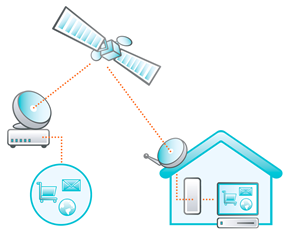
\includegraphics[scale=1]{Imagenes/Casa.png}
		\label{fig:Casa}
		%	\captionsetup{justification=raggedright,font={scriptsize,bf,it}}
		%	\caption*{fuente: \textcolor{
		%			Orange}{Tomada de Wikipedia}}
	\end{figure}
La reflexión es responsable del fenómeno de de multitrayectoria o Rayleigh y el de scattering. 

\subsection{Scattering como consecuencia de la reflexión}

El scattering es debido a las condiciones de la superficie sobre la cual cae una onda incidente, resulta un desorden de ondas son reflejadas en diferentes direcciones, como se muestra en la Figura \ref{fig:Refraccion}.
	
	\begin{figure}[h!]
		\captionsetup{justification = raggedright, singlelinecheck = false}
		\caption{Fenómeno de Scattering} 
		\centering
		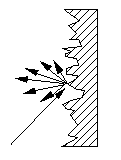
\includegraphics[scale=1]{Imagenes/Refraccion.png}
		\label{fig:Refraccion}
		%	\captionsetup{justification=raggedright,font={scriptsize,bf,it}}
		%	\caption*{fuente: \textcolor{
		%			Orange}{Tomada de Wikipedia}}
	\end{figure}



\subsection{La refracción}
Consiste en el cambio de dirección de una onda que se produce al pasar oblicuamente de un medio a otro de distinta densidad. Entre los usos o consecuencias de la refracción se tiene: \\

\begin{itemize}
	\item    La posibilidad de aprovechar este fenómeno para alcanzar puntos de comunicación tan lejanos que pueden estar más allá de la línea de vista aprovechando el paso por las capas atmosféricas con diferentes densidades.
	
%	\vspace{200px}
	\begin{figure}[h!]
		\captionsetup{justification = raggedright, singlelinecheck = false}
		\caption{Formas de refracción} 
		\centering
		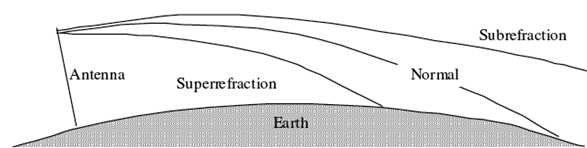
\includegraphics[scale=1]{Imagenes/Earth.png}
		\label{fig:Earth}
		%	\captionsetup{justification=raggedright,font={scriptsize,bf,it}}
		%	\caption*{fuente: \textcolor{
		%			Orange}{Tomada de Wikipedia}}
	\end{figure}
	\item  El uso de la ionosfera en sistemas de comunicación terrestres o espaciales.
	
	%\vspace{200px}
	\begin{figure}[h!]
		\captionsetup{justification = raggedright, singlelinecheck = false}
		\caption{El camino por refracción en función del ángulo de emisión} 
		\centering
		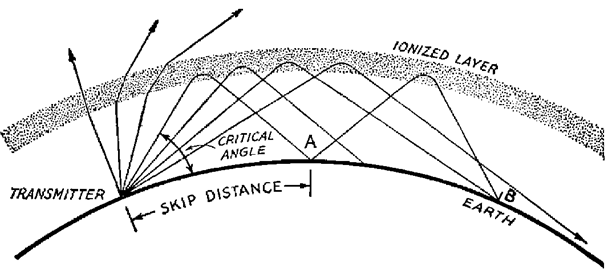
\includegraphics[scale=1]{Imagenes/Ionosfera.png}
		\label{fig:Ionosfera}
		%	\captionsetup{justification=raggedright,font={scriptsize,bf,it}}
		%	\caption*{fuente: \textcolor{
		%			Orange}{Tomada de Wikipedia}}
	\end{figure}
\end{itemize}


\subsection{La dispersión}
Ocurre cuando una onda atraviesa un medio que hace que diferentes longitudes de onda viajen a velocidades diferentes, lo cual hace también que cada longitud de onda tenga un ángulo de refracción diferente. En la Figura \ref{fig:Trian} se muestra un ejemplo para el caso de la luz. \\

\vspace{200px}
\begin{figure}[h!]
	\captionsetup{justification = raggedright, singlelinecheck = false}
	\caption{La Dispersión de la luz al pasar por un prisma} 
	\centering
	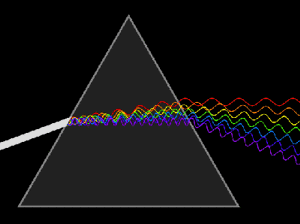
\includegraphics[scale=1]{Imagenes/Trian.png}
	\label{fig:Trian}
	%	\captionsetup{justification=raggedright,font={scriptsize,bf,it}}
	%	\caption*{fuente: \textcolor{
	%			Orange}{Tomada de Wikipedia}}
\end{figure}

Entre los usos o consecuencias de la dispersión se tiene: \\

\begin{itemize}
	\item  El efecto de la lluvia o la nubosidad en la calidad de las comunicaciones.
	
%	\vspace{200px}	
	\begin{figure}[h!]
		\captionsetup{justification = raggedright, singlelinecheck = false}
		\caption{Influencia de la lluvia en la dispesión} 
		\centering
		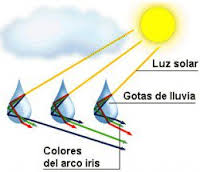
\includegraphics[scale=1]{Imagenes/lluvia.png}
		\label{fig:lluvia}
		%	\captionsetup{justification=raggedright,font={scriptsize,bf,it}}
		%	\caption*{fuente: \textcolor{
		%			Orange}{Tomada de Wikipedia}}
	\end{figure}
	
	\item  El surgimiento de interferencias indeseadas sobre una comunicación:
	
	\begin{figure}[h!]
		\captionsetup{justification = raggedright, singlelinecheck = false}
		\caption{Interferencias por Dispersión} 
		\centering
		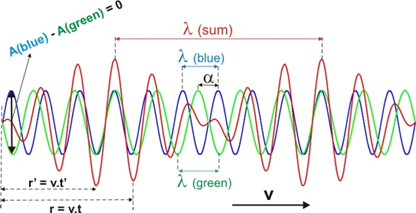
\includegraphics[scale=1]{Imagenes/Onda.png}
		\label{fig:Onda}
		%	\captionsetup{justification=raggedright,font={scriptsize,bf,it}}
		%	\caption*{fuente: \textcolor{
		%			Orange}{Tomada de Wikipedia}}
	\end{figure}
\end{itemize}
%\vspace{100px}
\subsection{La difracción}

%\vspace{5px}
\begin{figure}[h!]
	\captionsetup{justification = raggedright, singlelinecheck = false}
	\caption{La Difracción en las ondas de agua} 
	\centering
	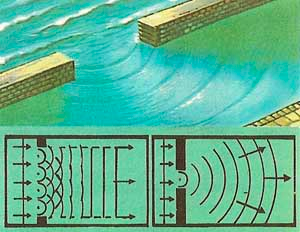
\includegraphics[scale=1]{Imagenes/Rio.png}
	\label{fig:Rio}
	%	\captionsetup{justification=raggedright,font={scriptsize,bf,it}}
	%	\caption*{fuente: \textcolor{
	%			Orange}{Tomada de Wikipedia}}
\end{figure}

Es la responsable del fenómeno conocido como sombra (shadowing), pues a un punto obstruido llega menos energía que a uno en línea de vista, como se muestra en la siguiente figura.

%	\vspace{200px}
\begin{figure}[h!]
	\captionsetup{justification = raggedright, singlelinecheck = false}
	\caption{La sombra como consecuencia de la difración} 
	\centering
	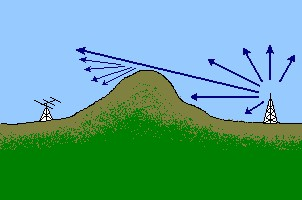
\includegraphics[scale=1]{Imagenes/Valle.png}
	\label{fig:Valle}
	%	\captionsetup{justification=raggedright,font={scriptsize,bf,it}}
	%	\caption*{fuente: \textcolor{
	%			Orange}{Tomada de Wikipedia}}
\end{figure}

\subsection{El Efecto Doppler}

Es el cambio de frecuencia que sufre una onda simplemente debido a la velocidad relativa entre los elementos que intervienen en la comunicación.\\

%\vspace{300px}
\begin{figure}[h!]
	\captionsetup{justification = raggedright, singlelinecheck = false}
	\caption{El Efecto Doppler} 
	\centering
	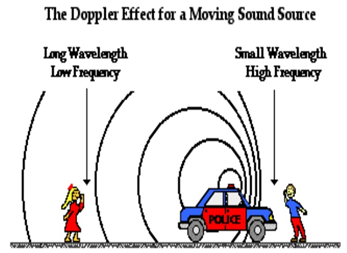
\includegraphics[scale=1]{Imagenes/Policia.png}
	\label{fig:Policia}
		\captionsetup{justification=raggedright,font={scriptsize,bf,it}}
		\caption*{fuente: \textcolor{
			Orange}{Wikipedia}}
\end{figure}

\textbf{Consecuencias del Efecto Doppler:} En un receptor digital basado en GNU Radio este efecto se traduce en que la constelación observada adquiere una velocidad proporcional a la frecuencia Doppler.

\section{La radio propagación}

La radiopropagación brinda herramientas para realizar planeación de coberturas de un sistema de radio comunicaciones. Sin embargo nuestro interés principal es conocer cómo los fenómenos de propagación pueden afectar a una señal que viaja por el canal y cuales pueden ser las medidas para contrarrestar esos efectos. \\

\subsection{La antena}
\textcolor{red}{Oscar reyes}
\textcolor{red}{[Falta. La idea es explicar lo suficiente como para que el estudiante sepa que aquí hay un elemento que no puede ignorar. Por ejemplo, el uso de una antena inadecuada puede hacer que no llegue señal, bien sea por los parámetros que la antena tiene o porque ese dañada. También puede ocurrir que no se esté apuntando hacia otras partes. Fuera de que el usuario debe tomar precauciones por la radiación que produce la antena y los posibles daños a la salud. Por lo menos debe saber si realmente está protegido. Para profundizar más, ofreceremos enlaces a la página web del libro.}\\ %\OR extensión?

La antena en el modo de transmisión puede ser vista como un conversor de una señal eléctrica a una señal electromagnética capaz de propagarse en forma de ondas electromagnéticas. Igualmente, en el modo de recepción representa una especie de sensor de las ondas electromagnéticas para expresarlas en forma eléctrica. Por sencillo que parezca esto, representa realmente la Teoría de Maxwell y su aplicación a la teoría de antenas, pero no es objetivo de este libro entrar a profundizar en estos temas. Lo que es importante tener en cuenta es que la antena tiene limitaciones expresadas principalmente en el cuanto a Ancho de Banda, su capacidad para enfocarse en una dirección, mejor conocida como la directividad de la antena o patrón de radiación de la antena y algunos coeficientes de rendimiento.\\

\subsubsection{La Potencia Isotrópica Radiada Equivalente - PIRE}
En los sistemas de Radiocomunicación, la Potencia Isotrópica Radiada Equivalente (PIRE) es la cantidad de potencia que emitiría una antena isotrópica teórica (es decir, aquella que distribuye la potencia exactamente igual en todas direcciones) para producir la densidad de potencia observada en la dirección de máxima ganancia de una antena. La PIRE tiene en cuenta las pérdidas de la línea de transmisión y en los conectores e incluye la ganancia de la antena. La PIRE se expresa habitualmente en decibelios respecto a una potencia de referencia emitida por una potencia de señal equivalente. La PIRE permite comparar emisores diferentes independientemente de su tipo, tamaño o forma. Conociendo la PIRE y la ganancia de la antena real es posible calcular la potencia real y los valores del campo electromagnético.



\begin{equation} \label{equ_pire}
PIRE=P_{T}-L_{c}+G_{a}	 				
\end{equation}

donde $ PIRE $ y $P_{T}$  (potencia del transmisor) son $dBm$, las pérdidas del cable ($L_{c}$) están en $d$, y la ganancia de la antena ( $G_{a})$  se expresa en $dBi$, relativos a la antena de referencia isotrópica.

El siguiente ejemplo utiliza dBm, aunque también es correcto utilizar dBW. Los Decibelios son una forma muy práctica de expresar la relación entre dos cantidades. dBm utiliza una referencia de 1 mW y dBW 1 W.

\begin{equation} \label{equ_dbm}
dBm=10\log \left({\frac {\text{potencia}}{1\,\mathrm {mW} }}\right) 				
\end{equation}

y

\begin{equation} \label{equ_dbw}
dBW=10\log \left({\frac {\text{potencia}}{1\,\mathrm {W} }}\right) 				
\end{equation}



Por ejemplo, una transmisión de 50 W es lo mismo que 17 dBW o 47 dBm.

\begin{equation} \label{equ_dbwdos}
\displaystyle 16.9897\,\mathrm {dBW} =10\log \left({\frac {50\,\mathrm {W} }{1\,\mathrm {W} }}\right) \\
\end{equation}

La PIRE se utiliza para estimar el área en el que la antena puede dar servicio y coordinar la radicación entre transmisores para que no se solapen las coberturas.
%%%%%%%%%%%%%%%%%%%%%%%%%%%%%%%%%%%%%%%%%%%%%%%%%%%

\subsection{La Densidad de Flujo de Potencia}

En un punto de interés, en campo lejano, la Densidad de Flujo de Potencia (PFD, del inglés Power Flux Density) está dada por el producto cruz entre los vectores $\overline{E}$ y $\overline{H}$:

\begin{equation} \label{equ_cuarenta_uno}
	 |\overline{S}|=|\overline{E} x \overline{H}|=|\overline{E} | |\overline{H}| sin \theta
\end{equation}

Donde $\overline{S}$ representa la PFD, $\overline{E}$  el campo eléctrico, $\overline{H}$ el campo magnético y $\theta$=90º el ángulo entre $\overline{E}$ y $\overline{H}$ para el caso del campo lejano. De modo que, para el campo lejano,  se puede reescribir  como: 

\begin{equation} \label{equ_cuarenta_dos}
	|\overline{S}|=|\overline{E} | |\overline{H}|
\end{equation}


Resulta importante apuntar que, desde el punto de vista de la propagación del campo eléctrico, el vacío (el espacio libre) tiene una impedancia conocida como impedancia característica del espacio libre y es igual a: 

\begin{equation} \label{equ_cuarenta_tres}
	 \eta_{0} = \dfrac{|\overline{E} |}{|\overline{H}|} = \sqrt{\dfrac{\mu_{0}}{\varepsilon_{0}}}= 120\pi \Omega \approx 337\Omega 
\end{equation}

Esta relación se conoce como la ley de Ohm para los campos electromagnéticos, donde $\mu_{0}=1,26 10-6H/m$ es la permeabilidad magnética del espacio libre; $\varepsilon_{0}=8,85 10-12F/m$ es la permitividad eléctrica del espacio libre. Como consecuencia, la PFD promediada guarda una relación con el valor RMS E de la intensidad del campo eléctrico $\overline{E}$ , en un Punto de interés  (PoI, del inglés Point of Interés), similar a la que existe entre la potencia promedio P de una señal de voltaje y su valor RMS: 

\begin{equation} \label{equ_cuarenta_cuatro}
	  S= \dfrac{E^{2}}{\varepsilon_{0}}
\end{equation}

En campo lejano es posible obtener el valor RMS H de la intensidad del campo magnético $\overline{H}$ a partir del eléctrico y viceversa de la siguiente manera:

\begin{equation} \label{equ_cuarenta_cinco}
	  H= \dfrac{E}{\varepsilon_{0}}, E=\varepsilon_{0}H
\end{equation}

Cuando se realizan mediciones de espectro, las emisiones pueden provenir de diferentes direcciones. Por eso, en algunos casos puede ser necesario conocer los aportes a E y H en las direcciones de las 3 direcciones del espacio físico, tridimensional:

\begin{equation} \label{equ_cuarenta_seis}
E = \sqrt{E_{x}^{2}+E_{y}^{2}+E_{z}^{2}} 
\end{equation}

\begin{equation} \label{equ_cuarenta_siete}
 H = \sqrt{H_{x}^{2}+H_{y}^{2}+H_{z}^{2}} 
\end{equation}

\subsection{Fenómeno de desvanecimiento. Pérdidas por Espacio Libre. Ecuación de Friss}

Se conoce como desvanecimiento en espacio libre (free space path loss) la pérdida de potencia captada por un receptor en función de la transmitida por un emisor, cuando no existe ningún obstáculo para la propagación, como ocurre en el cosmos o Espacio Libre (Free Space). Conocer la regla de cálculo de este tipo de pérdidas es de gran utilidad ya que sirven como una primera aproximación para las mediciones de la potencia que puede llegar a un receptor ubicado a una cierta distancia del emisor. \\



\subsubsection{La densidad de Flujo de Potencia en campo lejano}

Un caso teórico de enorme importancia consiste en el supuesto de contar con una fuente isotrópica que radia una potencia promedio $P_t$. La cuestión es que a medida que la onda se aleja a una distancia d, esa potencia se distribuye en el área de una  esfera $A$ de radio $d$ que se conforma alrededor de la fuente. Precisamente, como la potencia se distribuye en un área, se puede hablar de la Densidad de flujo de potencia $S_d$ por área.  Teniendo en cuenta que el área de la esfera es.\\

\begin{equation} \label{equ_cuarenta_ocho}
	 A_{es}= 4 \pi d^{2}
\end{equation}

La PFD es:

\begin{equation} \label{equ_cuarenta_nueve}
	S_{d}= \dfrac{P_t}{A_{es}}= \dfrac{P_t}{4 \pi d^{2}} Watt/m^{2}
\end{equation}

\subsubsection{El área efectiva de una antena }

En un área elemental de interés para la recepción $A_r (m^{2})$, como se muestra en la figura \ref{fig:Antena} , se recibe una potencia elemental $P_r$

$P_r= S_d A_r$

%\vspace{300px}
%	\setcounter{figure}{94}
\begin{figure}[h!]
	\captionsetup{justification = raggedright, singlelinecheck = false}
	\caption{Elemento de Área donde puede localizarse el receptor} 
	\centering
	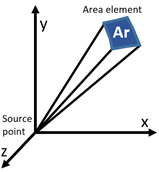
\includegraphics[scale=1.1]{Imagenes/Antena.png}
	\label{fig:Antena}
	%	\captionsetup{justification=raggedright,font={scriptsize,bf,it}}
	%	\caption*{fuente: \textcolor{
	%			Orange}{Tomada de Wikipedia}}
\end{figure}


Una antena, vista como un sensor, debe abarcar cierta área. Por esta razón, la capacidad de una antena para captar una potencia $P_r$ está asociada a un área que se conoce como el área efectiva Aeff de la antena o apertura efectiva de la antena.

\subsubsection{Una antena isotrópica} 

Una antena de recepción isotrópica ideal es aquella que irradia (o recibe) por igual en todas direcciones y tiene un área efectiva $A_{effiso}$ bien conocida que sirve como patrón para caracterizar otras antenas:

\begin{equation} \label{equ_cincuenta}
	A_{effiso} =\dfrac{\lambda^{2}}{4 \pi}= \frac{c^{2}}{4\pi f^{2}} 
\end{equation}

Así, el área efectiva está en función de la longitud de onda y disminuye conforme aumenta la frecuencia. Por esa razón, desde el punto de vista de una antena isotrópica, las ondas de mayor frecuencia se atenúan más rápidamente que las de menor. Por lo tanto, la potencia que puede captar una antena isotrópica es: \\

\begin{equation} \label{equ_cincuenta_uno}
	P_r= S_d A_{effiso}= S_d \dfrac{\lambda^{2}}{4 \pi} =  P_t \left(\dfrac{\lambda}{4 \pi d}\right)^{2}
\end{equation}

\subsubsection{Ecuación de Friis}

Es claro que a medida que una  señal de radio se propaga en la distancia, su energía se va esparciendo en un área cada vez mayor, lo cual va a ser percibido por un equipo receptor como un desvanecimiento, que en condiciones ideales, de espacio libre y usando antenas isotrópicas en transmisión y recepción, se expresa por el coeficiente:

\begin{equation} \label{equ_cincuenta_dos}
		 l_{fs}=  \left(\dfrac{4 \pi d}{\lambda} \right)  ^{2}
\end{equation}

Este coeficiente se conoce en inglés como Free Space Path Loss, en español como  Desvanecimiento en Espacio Libre o Pérdidas en Espacio Libre.\\
En función de la frecuencia tenemos que:

\begin{equation} \label{equ_cincuenta_tres}
	 l_{fs}=  \left(\dfrac{4 \pi df}{c} \right)  ^{2}
\end{equation}

Donde $c$ es la velocidad de la luz. \\
Muchas veces el Desvanecimiento en Espacio Libre se usa en dB. \\


\begin{equation} \label{equ_cincuenta_cuatro}
	 l_{fs}(dB)=  10log(lf_{s})
\end{equation}

\begin{equation} \label{equ_cincuenta_cinco}
	 l_{fs}(dB)=  20log\left(\dfrac{4\pi}{0.3(km/\mu seg)}\right)+ 20log(d(km)f(MHz))
\end{equation}

Entonces se obtiene la expresión más conocida para las pérdidas en espacio libre: \\
\begin{equation} \label{equ_cincuenta_seis}
	 l_{fs}(dB)=  32.4+20log(f)(MHz)+20log(d)[km]
\end{equation}

No hay que olvidar que aún con estos ajustes de ganancia, esta ecuación corresponde al caso ideal de propagación en espacio libre.  En un caso real, para las comunicaciones terrenales las pérdidas en espacio libre son apenas una referencia a la cual se suman otras pérdidas como las pérdidas por irregularidad del terreno o las pérdidas por otros aspectos como la altura del transmisor, la del receptor, si el ambiente de propagación que puede ser urbano, suburbano, rural, abierto o porque que hay tipos especiales de vegetación o falta de ella: \\

\begin{equation} \label{equ_cincuenta_siete}
	L(dB)=L_{reference}+L_{Terrain Irregularity}+L_{Environment}
\end{equation}

En condiciones de espacio libre, la potencia recibida se puede calcular como: \\

\begin{equation} \label{equ_cincuenta_ocho}
	 P_r=\frac{P_t}{l_{fs}}=P_t\left(\frac{\lambda}{4\pi d}\right)^{2}
\end{equation}

Si las antenas no son isotrópicas se les puede realizar ajuste, con lo cual se llega a la forma más común de la Ecuación de Friis:

\begin{equation} \label{equ_cincuenta_nueve}
	 P_r= P_t G_t G_r\frac{P_t}{l_{fs}}=P_t\left(\frac{\lambda}{4\pi d}\right)^{2}
\end{equation}

\textbf{Nota:} $G_r$ está multiplicando a la derecha, entonces está dividiendo a la izquierda, luego $\frac{P_r}{G_t}= \dfrac{P_tG_r}{l_{sf}}$. Eso es correcto, pues la ganancia en la parte receptor contribuye a elevar el área efectiva de la antena receptora y esa área está a la derecha de la ecuación.
Entonces la potencia recibida se calcula como: \\

\begin{equation} \label{equ_sesenta}
	P_r(dB)=P_t(dB)+G_t(dB)+G_r(dB-L(dB)
\end{equation}

\subsection{Propagación en Línea de Vista. Distribución de Rice}
En el mundo real, la potencia que se recibe está oscilando todo el tiempo y el comportamiento de esas oscilaciones depende de varios factores. Uno de ellos es que la recepción se realice en línea de vista (LOS, del inglés Line of Sight), donde, aunque influyen muchos fenómenos de las ondas, predomina la señal que llega directamente de la antena transmisora, pero es influenciada por débiles señales que llegan reflejadas de diferentes obstáculos. \\
%\vspace{200px}
\begin{figure}[h!]
	\captionsetup{justification = raggedright, singlelinecheck = false}
	\caption{Fenómeno de Multitrayectoria} 
	\centering
	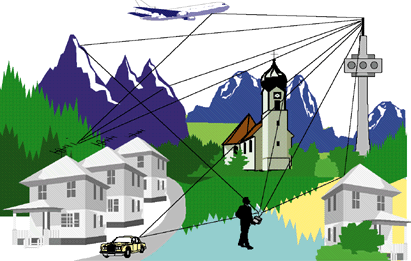
\includegraphics[scale=1]{Imagenes/Edificio.png}
	\label{fig:Edificio}
	%	\captionsetup{justification=raggedright,font={scriptsize,bf,it}}
	%	\caption*{fuente: \textcolor{
	%			Orange}{Tomada de Wikipedia}}
\end{figure}

En la siguiente figura se muestra la imagen que resulta al medir la potencia de la señal RF para este caso. \\
%\vspace{100px}
\begin{figure}[h!]
	\captionsetup{justification = raggedright, singlelinecheck = false}
	\caption{Nivel de potencia medida en LOS} 
	\centering
	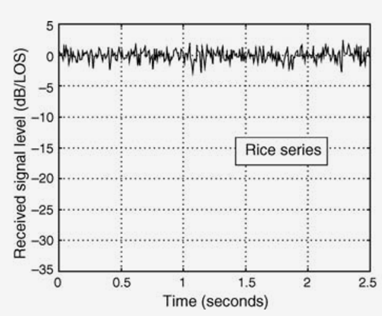
\includegraphics[scale=1]{Imagenes/Medidor.png}
	\label{fig:Medidor}
		\captionsetup{justification=raggedright,font={scriptsize,bf,it}}
		\caption*{fuente: Tomado de F. Pérez Fontán\textbf{Nota:}Esta no es la señal recibida sino lo que entrega un medidor de nivel de potencia} 
\end{figure}

Desde el punto de vista de los Procesos estocásticos, el nivel de señal que se recibe en línea de vista sigue la distribución de Rice.\\

El efecto de Rice se observa no solo en LOS, sino también en algunos casos ocurre en No Línea de Vista (NLOS), por ejemplo, cuando un obstáculo puede ser visto como un fuerte reflector de la señal, lo cual ocurre a menudo en las comunicaciones móviles cuando la señal llega reflejada de una superficie suave de un edificio que si tiene LOS. \\

\subsection{Pérdidas Propagación en Línea de Vista. Distribución de Rice}

Cuando no hay línea de vista (NLOS), en el nivel de señal recibido predominan los débiles aportes de energía que se reciben de manera indirecta, principalmente por el efecto de multitrayectoria, es decir la multitud de ondas que llegan al receptor, recorriendo diferentes distancias, debido al efecto de la reflexión que las  ondas sufren al encontrarse con diferentes obstáculos en su propagación. Estos obstáculos pueden ser edificios, señales de tráfico, árboles, personas y hasta gatos. La suma de las señales que llegan de esos obstáculos causa en el receptor distorsiones tanto constructivas como destructivas. \\

Cuando predomina el efecto de multitrayectoria, la señal RF medida en el receptor muestra una combinación de variaciones rápidas (Fast Fading) y lentas (Slow Fading), como se muestra en la figura siguiente. \\ 

%\vspace{200px}
\begin{figure}[h!]
	\captionsetup{justification = raggedright, singlelinecheck = false}
	\caption{Niveles de potencia medidos en un punto donde se presenta el Efecto de Rayleigh} 
	\centering
	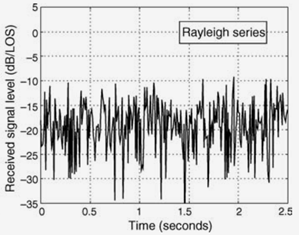
\includegraphics[scale=1]{Imagenes/Rayleigh.png}
	\label{fig:Rayleigh}
	\captionsetup{justification=raggedright,font={scriptsize,bf,it}}
		\caption*{Fuente: Tomado de F. Pérez Fontán. Nota: esta no es la señal recibida sino lo que entrega un medidor de nivel de potencia} 
\end{figure}

Pero el efecto de Rayleigh no solo se observa en condiciones de NLOS, también se observa en un vehículo que se mantiene en LOS, alejándose de la fuente, mientras se desplaza por una zona rural con geografía variable, como se muestra en la siguiente figura. \\

\vspace{200px}
\begin{figure}[h!]
	\captionsetup{justification = raggedright, singlelinecheck = false}
	\caption{Efecto de Rayleigh en un caso de LOS} 
	\centering
	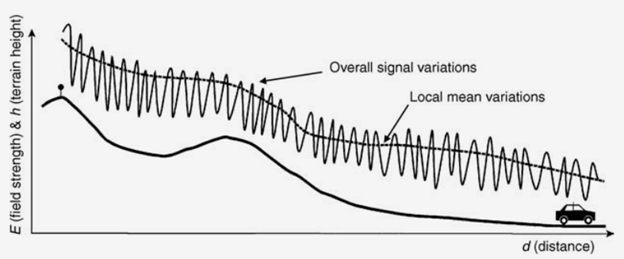
\includegraphics[scale=1]{Imagenes/Field.png}
	\label{fig:Field}
	\captionsetup{justification=raggedright,font={scriptsize,bf,it}}
	\caption*{Fuente: Tomado de F. Pérez Fontán. Nota: Esta no es la señal recibida sino lo que entrega un medidor de nivel de potencia. En esta figura no se muestra el desvanecimiento por la distancia, que puede compensarse mediante un sistema de amplificación automática.} 
\end{figure}

Las variaciones rápidas (Fast Fading or Fast Variations or short term variations) son debidas al efecto de multitrayectoria en sí, mientras que las lentas (Slow Fading or Slow Variations or long-term variations) son debidas principalmente efecto de desvanecimiento por sombra (shadowing), el cual, a su vez es una consecuencia de refracción de las ondas con respecto a las montañas y otros obstáculos. El anterior es el peor escenario, se encuentra en ambientes urbanos densos de altas edificaciones, pero también en ambientes rurales donde la señal es obstruida por densa masa de árboles. La siguiente figura muestra lo que pasaría si las variaciones lentas son promediadas, (parte izquierda) y las variaciones rápidas que resultan al restar a la señal las variaciones lentas (parte derecha). \\

\begin{figure}[h!]
	\captionsetup{justification = raggedright, singlelinecheck = false}
	\caption{El Desvanecimiento lento} 
	\centering
	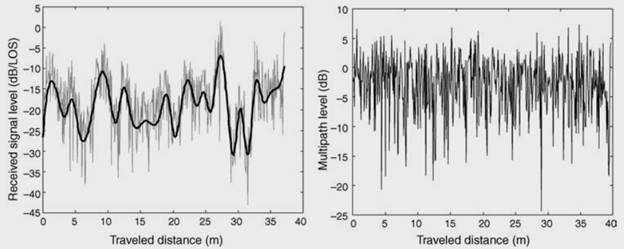
\includegraphics[scale=1]{Imagenes/Distancia.png}
	\label{fig:Distancia}
	\captionsetup{justification=raggedright,font={scriptsize,bf,it}}
	\caption*{Fuente: tomado de F. Pérez Fontán} 
\end{figure}

\section{Equipo de Laboratorio y de medida}

\subsection{El osciloscopio}
\textcolor{red}{[Falta: Oscar Reyes]} % \OR Algún osciloscopio en particular? Qué tan general??

[Falta. La idea es brindar una pequeña explicación y un enlace a la pagina web para que vean un curso sobre el uso correcto del equipo. Hay que dejar claro, que al igual que los USRP son equipos que hay que conocer muy bien y darle un buen uso para que no se dañen. Es importante incluir unas recomendaciones de uso aquí.]

\subsection{El Analizador de Espectros}

Aunque se dice que el ERE es un recurso intangible, que no se puede ver, ni oler, ni pesar, en realidad es posible apreciarlo mediante el uso de un Analizador de Espectros.\\

El Analizador de espectros se basa en el uso de un banco de filtros, cada uno de los cuales está acotado a un ancho de banda lo más angosta posible centrado en una frecuencia diferente a los demás, de modo que entre todos los filtros sea posible cubrir un ancho de banda de interés, centrado en una cierta frecuencia intermedia (FI). El uso de un receptor superheterodino es clave para poder mover a la FI el espectro de la señal que se desea analizar. Una pantalla toma la salida de cada filtro para crear la imágen espectral que consiste en amplitudes de señal distribuidas sobre el eje de las frecuencias. El espectro que muestra el Analizador de espectros es dinámico ya que corresponde a al comportamiento instantáneo de una señal, a diferencia de los métodos teóricos usados para obtener el espectro, donde una señal es muchas veces analizada en toda su extensión. También es posible obtener un espectro promediado y un espectro pico como imágenes algo más estáticas. \\

Los analizadores de espectros pueden ser construidos también con tecnología digital que imita al banco de filtros por lo que tienen la misma apariencia.\\
\textcolor{red}{[Falta: Oscar Reyes]} % \OR qué se espera, qué extensión? enfocado a uso, a estructura....?


\subsection{El Analizador Vectorial de Redes}
\textcolor{red}{Falta:Oscar reyes }\\


\subsection{El Generador Vectorial de Señales}
\textcolor{red}{Falta:Oscar reyes }\\
\subsection{El Analizador Vectorial de Señales}
\textcolor{red}{Falta: Oscar reyes }\\


\subsection{El Analizador Vectorial de Señales}
\textcolor{red}{Falta: Oscar Reyes }\\

\subsection{Medidor de RNI}
\textcolor{red}{Falta: Oscar Reyes}\\

\section{Medición de potencia propagada}

El espacio libre se refiere al caso ideal en que las ondas se propagan libres de cualquier obstáculo como sucedería por ejemplo en el cosmos. Pero tiene una gran utilidad también para condiciones terrestres, pues brinda la posibilidad de realizar una aproximación gruesa, que puede ser complementada con factores terrestres si resulta necesario obtener cálculos más precisos. \\

\subsection{Valor RMS y Potencia Promedio}

En la práctica, aunque el equipo de medición se ubique en un punto de interés (PoI) fijo, la amplitud de las ondas que inciden en el equipo varían aleatoriamente, debido a la información que transportan y a todos los fenómenos que ocurren en el canal inalámbrico. Consecuentemente varía en el tiempo la señal de voltaje que entrega la antena del equipo de medición. Por esta razòn, es necesario usar promedios de tiempo. Resulta entonces pertinente recordar la definición de valor RMS que uno de esos promedios aplicados a una señal aleatoria de voltaje v(t): \\

\begin{equation} \label{equ_sesenta_uno}
	 V_{RMS} = \lim_{Taver \to \infty} \sqrt{\dfrac{1}{Taver} \int_{0}^{Taver} |V(t)|^{2} dt} 
\end{equation}

Otro promedio de tiempo importante es el de potencia promedio, que se puede obtener a partir del valor RMS asì: \\

\begin{equation} \label{equ_sesenta_dos}
	 P = \dfrac{{V_{RMS}}^{2}}{Z} = \lim_{Taver \to \infty} \dfrac{1}{Z Taver} \int_{0}^{Taver} |V(t)|^{2} dt 
\end{equation}

Donde Z es la impedancia del medio en el cual viaja la señal . \\

\subsection{Campo cercano versus campo lejano. }

En la radio propagación de las ondas electromagnéticas se distinguen el campo cercano y el campo lejano. Lo importante a tener en cuenta en las mediciones es que, a una distancia mayor a 3 longitudes de onda, es posible considerar que el frente de una onda electromagnética que puede ser capturado por una antena es plano y los campos eléctricos y el magnético son ortogonales entre sí. No ocurre lo mismo a distancias menores y, por lo tanto, se requieren equipos especializados para la medición. El primer caso corresponde al campo lejano y el segundo al cercano. Los equipos de medición que provee la industria para frecuencias altas en campo lejano permiten medir el campo eléctrico E(V/m) o el campo magnético H(A/m) o la densidad de flujo de potencia $S(W/m^{2})$. \\

\subsection{Factor de antena} 

Una de las grandes dificultades para la realización de trabajos de campo radica en el diseño de un equipo capaz de medir la intensidad de un campo eléctrico incidente $e_i (t)$ en un PoI, empleando un receptor de ondas RF y una antena. La antena es usada como un sensor de la intensidad del campo eléctrico en el PoI, o más bien como un transductor de ese campo a una señal eléctrica aleatoria de voltaje $v_r (t)$ que tiene un valor RMS $V_r$. De modo que la potencia promedio es:   \\


\begin{equation} \label{equ_sesenta_tres}
	 P_R= \dfrac{V_r^{2}}{Z_{Ant}}
\end{equation}

Donde $Z_{Ant}$ es impedancia de la antena receptora. El Factor (AF) de la antena receptora es precisamente el coeficiente de proporcionalidad entre  $E_i$ y $V_r$:

\begin{equation} \label{equ_sesenta_cuatro}
	  A_{fR} = \dfrac{E_i}{V_r}
\end{equation}

Por esta razón es necesario conocer el AF para determinar la intensidad del campo eléctrico incidente a partir $V_r$. Además, con los conceptos ya vistos, puede deducirse que  $V_r$ está relacionado con el área efectiva de la antena así: \\

\begin{equation} \label{equ_sesenta_cinco}
	 \dfrac{{V_{r}}^{2}}{Z_{Ant}} = S_{r} A_{eff}= \dfrac{{E_{i}}^{2}}{120 \pi} * \dfrac{\lambda^{2}}{4\pi} G_{r}
\end{equation}

Por lo tanto, el factor de antena puede hallarse a partir de los parámetros de la antena y es función de la longitud de onda: \\
        
\begin{equation} \label{equ_sesenta_sies}
	  A_{fR} = \dfrac{E_i}{V_r} = \sqrt{\dfrac{480\pi^{2}}{Z_{Ant} \lambda^{2}G_{r}}}
\end{equation}

Esta fórmula sugiere conocer simplemente la ganancia de la antena receptora y la impedancia de la antena, mientras se hace variar la frecuencia o la longitud de onda en el rango de interés. También es posible encontrar una expresión para el factor de antena a partir de la potencia transmitida así: \\

\begin{equation} \label{equ_sesenta_siete}
S_{r}=\dfrac{P_{r}}{A_{eff}}= \dfrac{P_{t}G_{t}G_{r}}{A_{eff}} (\dfrac{\lambda}{4 \pi r})^{2}=\frac{P_{t}G_{t}}{4\pi r^{2}} 
\end{equation}

\begin{equation} \label{equ_sesenta_ocho}
{E_{i}}^{2} = S_{r}120\pi =30 \dfrac{P_{t} G_{t}}{r^{2}}
\end{equation}

Sustituyendo en $A_{fR} = \dfrac{1}{V_r}\sqrt{30P_{r}G_{t}}$ Esta fórmula sugiere la realización de un experimento usando un transmisor de potencia y ganancia conocida, y ubicando un receptor a una distancia $r$ también conocida, para medir $V_r$ y calcular el factor de antena según  \textcolor{orange}{(21)}. \\

La figura \ref{fig:Factor-antena} resumen las relaciones de mayor interés, donde se observa que: la antena transmisora también tiene un factor de antena $A_{fT}$, el cual también puede entrar a jugar un papel importante en las mediciones. \\ 

%\vspace{200px}
%\setcounter{figure}{126}
\begin{figure}[h!]
	\captionsetup{justification = raggedright, singlelinecheck = false}
	\caption{El factor de antena en la práctica} 
	\centering
	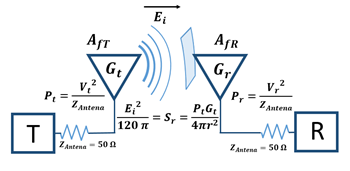
\includegraphics[scale=1]{Imagenes/Factor-antena.png}
	\label{fig:Factor-antena}
	%	\captionsetup{justification=raggedright,font={scriptsize,bf,it}}
	%	\caption*{fuente: \textcolor{
	%			Orange}{Tomada de Wikipedia}}
\end{figure}

\subsection{Parámetros S11 de las antenas}

El parámetro $S_{11}$ de una antena puede jugar también un papel importante en las mediciones de RNI. En este sentido, lo que debe tenerse en cuenta es que $S_{11}$ representa la relación entre la potencia reflejada por la antena u la aceptada y por eso se conoce también como coeficiente de reflexión o pérdidas de retorno de la antena. Por ejemplo, si $S_{11}=0dB$, toda la potencia es reflejada de la antena y nada es recibido. Pero si $S_{11}=-10 dB$ significa que si llegan 3 dB a la antena, -7dB es lo reflejado por la antena y lo demás es lo aceptado. 

\section{El Espectro Radioeléctrico}
El espectro radioeléctrico (ERE) es un término usado principalmente por las autoridades para hacer referencia a ese valioso recurso que permite el desarrollo de las comunicaciones inalámbricas.
Existen dos tipos de autoridades: las nacionales y las internacionales. A nivel internacional se tiene la Unión Internacional de Telecomunicaciones (UIT), donde se encuentra el sector de radiocomunicaciones (UIT-R). Las principales normas que \
rigen el ERE a nivel internacional están plasmadas en un acuerdo de carácter vinculante para todos los piases conocido como el Reglamento Internacional de Radio (RR, del inglés, Radio Regulations). A nivel de cada país, se tiene un documento que adapta el RR a las condiciones del \
país, en el caso de Colombia se conoce como el CNAB (Cuadro Nacional de Atribución de Bandas de Frecuencia). A continuación se resaltan la información del RR que resulta relevante para los propósitos del presente libro.

\subsection{Clasificación de las ondas de radio}

\textcolor{red}{[Falta. la idea es mostrar que las ondas electromagnéticas tienen las mismas cualidades de cualquier onda, pero que también hay aspectos especiales como:}  \\
 
 \begin{itemize}
	
	\item  No necesitan de un medio. El medio es el vació\\
    \item  La ecuación de Friss, que depende de la frecencia y la velocidad de la luz.
    \item  Que las ondas de radio, son en realidad una porción del espectro electromagnético.\\
    \item  Que todo lo anterior hace que sobre el planeta tierra las ondas tengan diferentes formas de propagación como: la ionosfera, en forma curvada, en línea recta, las espaciales, usando satélites, etc.\\
    \item  Que el ERE tienen una clasificación global en: ELF, SLF, ULF, VLF,LF, MF, HF, VHF, UHF, SHF, EHF]. tambien la clasificación en términos de la logitud de ondas como: ondas, larga, onda corta, etc.\\
\end{itemize}

\subsection{Gestión Internacional del Espectro}
\textcolor{red}{Esta es una buena fuente: https://www.itu.int/en/ITU-D/Regional-Presence/Americas/Documents/EVENTS/2016/15532-MX/D1-S2-1.pdf}
\subsubsection{La UIT y la UIT-R}

\textcolor{red}{Falta. La idea es presentar un resumen y luego mostrar enlaces a fuentes más completas.
NOTA: solo incluir no que un estudiante requiere para el curso. Lo demás, solo se referencia.}

\subsubsection{El Reglamento de Radiocomunicaciones}

\subsubsection{Los servicios de radiocomunicaciones}

El RR define ante todo los diferentes servicios de radio, las bandas de frecuencias que tienen asignadas y las condiciones en que pueden usar esas bandas. son 2 los grandes tipos de servicios:
    
\begin{itemize}
	\item   Terrenales. Son los que tienen lugar en el planeta tierra. Son 3:
    
    \begin{itemize}
	    \item  Servicios terrestres.
        \item  Servicios aeronáuticos.
        \item  Servicios marítimos.
    \end{itemize}
    
    \item  Espaciales. Los que tienen lugar fuera del planeta.
    
    	\begin{itemize}
	    	\item  Servicios satelitales
        	\item  Otros.
    	\end{itemize}
 
 	\item  Cada uno de los anteriores servicios pueden ser de tipo:
		\begin{itemize}
			\item  Servicio Fijo
    		\item  Servicio móvil
		\end{itemize}
\end{itemize}        

Para conocer con mayor profundidad estos temas, puede consultar los materiales disponibles en línea así:
\begin{itemize}
	\item   Sitio Web del libro, sección ERE 
	\item  Este es el enlace directo:
	\url{https://sites.google.com/saber.uis.edu.co/Libro/m/ERE}
\end{itemize}

\subsection{La Gestión Nacional del especto}

\textcolor{red}{Falta. La idea es presentar un resumen y enlaces a las fuentes disponibles. Es importante que estudiante conozca: las autoridades de regulación,las principales leyes y normas, pero sobre el todo el Cuadro Nacional de Atribución de Bandas de Frecuencia (CNABF), también las herramientas de consulta disponibles para conocer la ocupación del ERE.} \\

\textbf{NOTA: solo incluir no que un estudiante requiere para el curso. Lo demás, solo se referencia} \\

\subsubsection{El Ecosistema de la gestión del ERE}
\subsubsection{Autoridades de regulación}
\subsubsection{El CNABF}

%%%%%%%%%%%%%%%%%%%%%%%%%%%%%%%%%%%%%%%%%%

\section{Los modelos de capas para representar sistemas de comunicaciones}

Cualquier sistema de comunicaciones, por muy complejo que parezca, puede ser fácilmente representado mediante un modelo de capas- Esto aplica no solo en las telecomunicaciones, sino en cualquier otro sistema. Esto es debido a que, por naturaleza, la comunicación se da de manera elemental a diferentes niveles. Por ejemplo, en una empresa que vende artículos nacionales e importados pueden darse los siguientes niveles de comunicación, la que se da entre: el vendedor y el cliente; los vendedores y su jefe de ventas; los jefes de venta y su gerente; el gerente y las empresas proveedoras. En cada caso, se usa una forma especial de comunicación que puede involucrar formas de relación, términos especiales y hasta temas especiales.\\

En uso de modelos de capas en el presente libro cobra sentido por la gran cantidad de elementos que pueden llegar a formar parte de un sistema de radiocomunicaciones. Las ventajas se pueden resumir en los siguientes puntos. Permite:\\

\begin{itemize}
	\item[$\bullet$] Ordenar los elementos del sistema. Cuando no se usan capas, los componentes de un sistema de comunicaciones se parece a un ejército en el campo de batalla, donde todo funciona bien, pero resulta dificil de comprender cómo operan los diferentes mandos. Al usar el modelo de capas el sistema de comunicaciones se parece más bien a un desfile militar, donde al frente están los generales, luego los coroneles y así sucesivamente hasta llegar a los soldados.  
	\item  Reducir cuando sea necesario, el número de elementos del sistema, por ejemplo agrupando elementos en capas que encierran un mayor grupo de funcionalidades
    \item[$\bullet$] Construir un sistema funcional con funciones elementales, pero que puede ir creciendo con nuevas capas hasta llegar a ser tan complejo como sea necesario.
    \item[$\bullet$] Probar las funcionalidades de un sistema a nivel de una o algunas capas. Esto equivale a decir que es posible aislar algunas capas del sistema de comunicaciones con el fin de realizar cualquier tipo de pruebas, por ejemplo, para determinar en qué capa se puede estar presentando una falla.
\end{itemize}

Existen modelos de capas estandarizados, muy bien documentados que pueden ser usados para intercambiar ideas y conocimientos entre ingenieros y demás expertos en telecomunicaciones. Ejemplo de ellos son:
\begin{itemize}
	\item[$\bullet$] \textbf{El modelo OSI} Explicar los sistemas de comunicaciones de datos usando ocho capas. Así, un sistema particular de datos puede tener más o menos número de capas, pero a la hora de llevarlo a una discusión, siempre resulta posible presentar el sistema como el compuesto de ocho capas.
    \item[$\bullet$] \textbf{El modelo IP} IP se refiere al Protocolo de Internet, del inglés Internet Protocol. Se refiere a todo el conjunto de protocolos que se usan en las redes IP.
    \item[$\bullet$] \textbf{Otros.} La Unión Internacional de Telecomunicaciones (UIT) usa modelos para explicar diferentes sistemas de comunicaciones, como por el ejemplo para explicar el sistema de Telecomunicaciones Móviles internacionales (IMT, del inglés International Telecommunication Union), el Internet de las cosas (IoT, del inglés Internet of Things).
\end{itemize}

Los que usaremos en el presente libro no son modelos de capas recocidos, simplemente adaptados a nuestras necesidades que algunas veces son de diseño otras de documentación o simplemente de tipo pedagógico. \\

Para comenzar, vamos a revisar el modelo de capas que corresponde al sistema de comunicaciones que se da en el transporte aéreo. Con la creación de las aeronaves, se creó el sistema más sencillo usado en el transporte aéreo: la posibilidad de enlazar dos ciudades. \\
El modelo de capas que representa esta posibilidad es el que se tiene en la Figura \ref{fig:modelo_aviacion}. El avión aprovecha un pequeño corredor del Espacio Aéreo; en el aeropuerto convergen las personas y las aeronaves. \\

%\vspace{200px}
\begin{figure}[h!]
	\captionsetup{justification = raggedright, singlelinecheck = false}
	\caption{Modelo de capas para el transporte aéreo entre dos ciudades} 
	\centering
	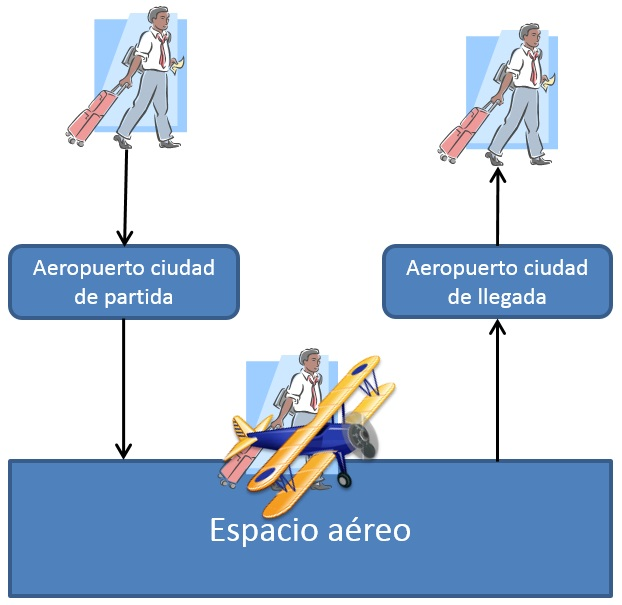
\includegraphics[scale=0.6]{Imagenes/modelo_aviacion}
	\label{fig:modelo_aviacion}
	%		\captionsetup{justification=raggedright,font={scriptsize,bf,it}}
	%		\caption*{fuente: http://superkuh.com/rtlsdr.html}
\end{figure}

Con el tiempo, ese sistema de comunicación evolucionó hasta convertirse en una compleja red que une miles de ciudades, como la que aparece en Figura \ref{fig:AirTrafficNetwork}, siempre respetando los lineamientos que imponen las autoridades encargadas de la administración del espacio aéreo. \\

%\vspace{200px}

\begin{figure}[h!]
	\captionsetup{justification = raggedright, singlelinecheck = false}
	\caption{Red de Transporte Aéreo} 
	\centering
	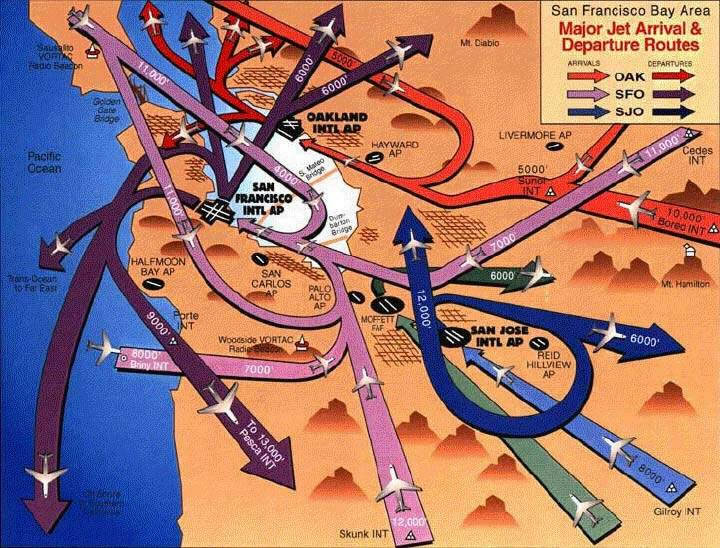
\includegraphics[scale=0.4]{Imagenes/AirTrafficNetwork}
	\label{fig:AirTrafficNetwork}
	\captionsetup{justification=raggedright,font={scriptsize,bf,it}}
	\caption*{fuente: http://https://www.paloaltoonline.com/}
\end{figure}

%\vspace{200px}
Las redes son mantenidas especialmente por las compañías aéreas. Ellas se apoyan en las capacidades que les ofrecen los aeropuertos y las autoridades aeronáuticas para ofrecer al pasajero la posibilidad de viajar desde cualquier punto a cualquier otro punto. Basta con que el pasajero muestre el ticket o pasaje para que cualquier oficina de su compañía de aviación, en cualquier país reconozca al pasajero, su origen y destino. Este complejo mecanismo se resume en un simple modelo de capas como el que se presenta en la Figura \ref{fig:modelo_aviacion_red}. \\

%\vspace{200px}
\begin{figure}[h!]
	\captionsetup{justification = raggedright, singlelinecheck = false}
	\caption{Red de Transporte Aéreo} 
	\centering
	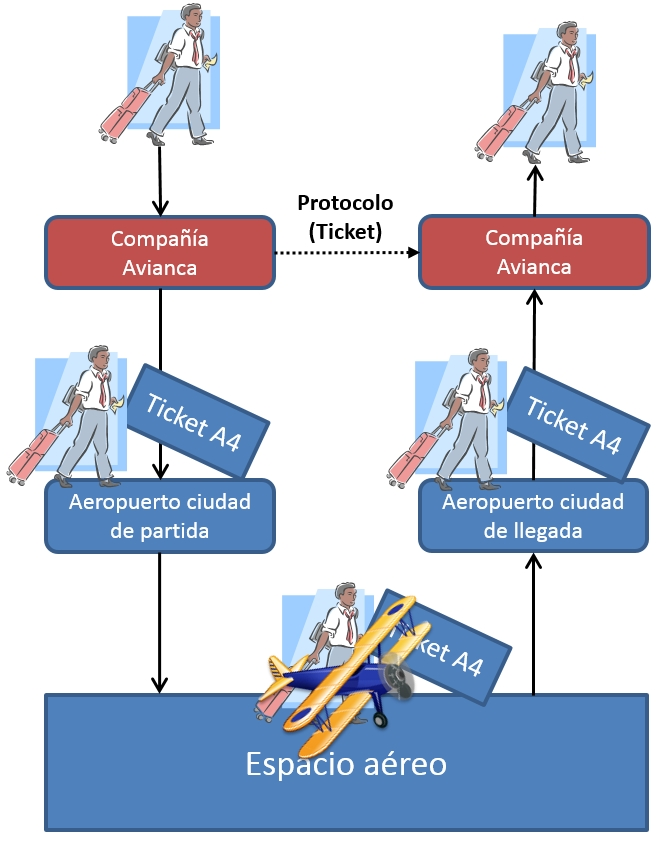
\includegraphics[scale=0.4]{Imagenes/modelo_aviacion_red}
	\label{fig:modelo_aviacion_red}
\end{figure}

En fin de cuentas, todo sistema de comunicación comienza por la conquista de un recurso para la comunicación. En las telecomunicaciones, los recursos más usados son las líneas de cobre, la fibra óptica, el espectro radioléctrico (ERE) y la luz, como es el caso de los sistemas de comunicaciones conocidos como Free Space Optics. Pero nada nos limita a pensar en otras posibilidades como el uso del ultrasonido e incluso no sería descabellado llegar descubrir información que viaja sobre las ondas gravitacionales que se desplazan por el universo.\\

En la Figura \ref{fig:CapasV1} se tiene un modelo de capas para el caso en que se usa el ERE. \\

%\vspace{200px}
\begin{figure}[h!]
	\captionsetup{justification = raggedright, singlelinecheck = false}
	\caption{Modelo de capas para un sistema de comunicaciones inalámbricas en red} 
	\centering
	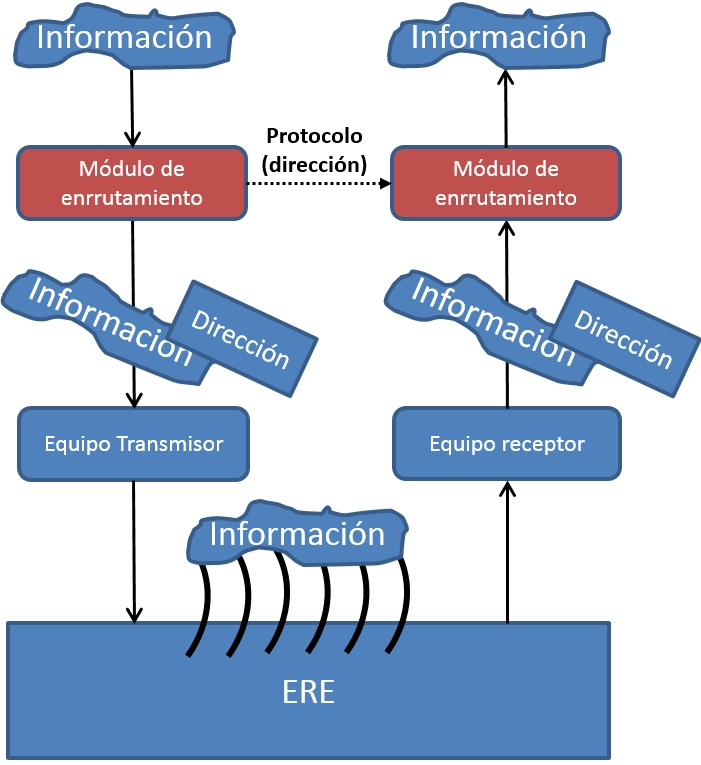
\includegraphics[scale=0.6]{Imagenes/CapasV1}
	\label{fig:CapasV1}
	%		\captionsetup{justification=raggedright,font={scriptsize,bf,it}}
	%		\caption*{fuente: http://superkuh.com/rtlsdr.html}
\end{figure}

Algunos conceptos importantes para este modelo son:   

\begin{itemize}
	\item  \textbf{Las ondas electromagnéticas:} Son el vehículo que hace uso del ERE para conducir información mediante la modulación de uno de sus parámetros. Claro está que en las radio comunicaciones solo se usan las ondas electromagnéticas que se encuentran en una banda del espectro conocida como el espectro radio eléctrico. Se trata de la banda comprendida entre 30 kHz y 300 GHz.
    \item  \textbf{ La modulación:} Consiste en el proceso de montar la información sobre algún medio de comunicación. En el caso de las radio comunicaciones, la información puede montarse sobre la onda en forma forma de variaciones de la amplitud de la onda, como cuando una persona usa su linterna, en cuna cueva para enviar mensajes a un compañero variando la intensidad de la luz. Pero también es posible hacer que la información viaje en forma de variaciones de la frecuencia o de la fase de la onda. 
    \item  \textbf{La Modulación de amplitud (AM):} Se da cuando la información viaja sobre una portadora en forma de variaciones de amplitud.
    \item  \textbf{Modulación de Frecuencia (FM):} Es el nombre que toma el método de modulación que usa la frecuencia de la onda portadora para llevar información.
    \item  \textbf{Modulación de Fase (PM):} Es el tercer método de modulación de una onda portadora y consiste en la posibilidad de hacer que la información viaje en forma de variaciones de la fase de la onda portadora.
\end{itemize}

Como en el caso del transporte aéreo, se ha introducido un módulo de enrrutamiento para que el modelo corresponda al de un sistema de comunicaciones en red. Algunos elementos de un modelo de capas son los siguientes:

\begin{itemize}
	\item  \textbf{Entidades pares:} En cada capa se tiene un módulo en el transmisor que hace pareja con un módulo en el receptor, esto es lo que se conoce como entidades pares.
    \item  \textbf{Protocolo:} corresponde a todo aquello que pueda ser usado entre las entidades pares para entenderse mutuamente. Por ejemplo, el módulo de enrrutamiento en la parte transmisora puede agregar a la información una etiqueta con la dirección de destino. El mismo módulo en en receptor leer esa dirección, para poder tomar una decisión que puede ser la de extraer la información para entregarla o la de encaminar esa información hacia otro destino.
    \item  \textbf{Canal:} se refiere aquello que se usa como medio para que viaje la información desde un origen hasta un destino. Es justo aquello que plantea los principales retos a un sistema de comunicaciones. Cada caso particular puede tener su propio canal. Así, en las radiocomunicaciones punto a punto el canal está usualmente representado por una banda concreta del ERE, pero limitada al espacio geográfico y al duración que corresponda según las normas para el sistema de comunicaciones dado. El canal inalámbrico representa enormes retos para los sistemas de comunicaciones pues el proceso de transmisión y recepción no solo deben sortear la necesidad de emitir y recibir ondas de radio sino la de considerar los diferentes fenómenos que esas ondas pueden sufrir en su propagación. 
\end{itemize}

La Figura \ref{fig:ModeloRadiodifusion} muestra el modelo de capas que podría ser usado para explicar el funcionamiento de la radio difusión. \\

\vspace{300px}
\begin{figure}[h!]
	\captionsetup{justification = raggedright, singlelinecheck = false}
	\caption{Modelo de capas para la radio difusión} 
	\centering
	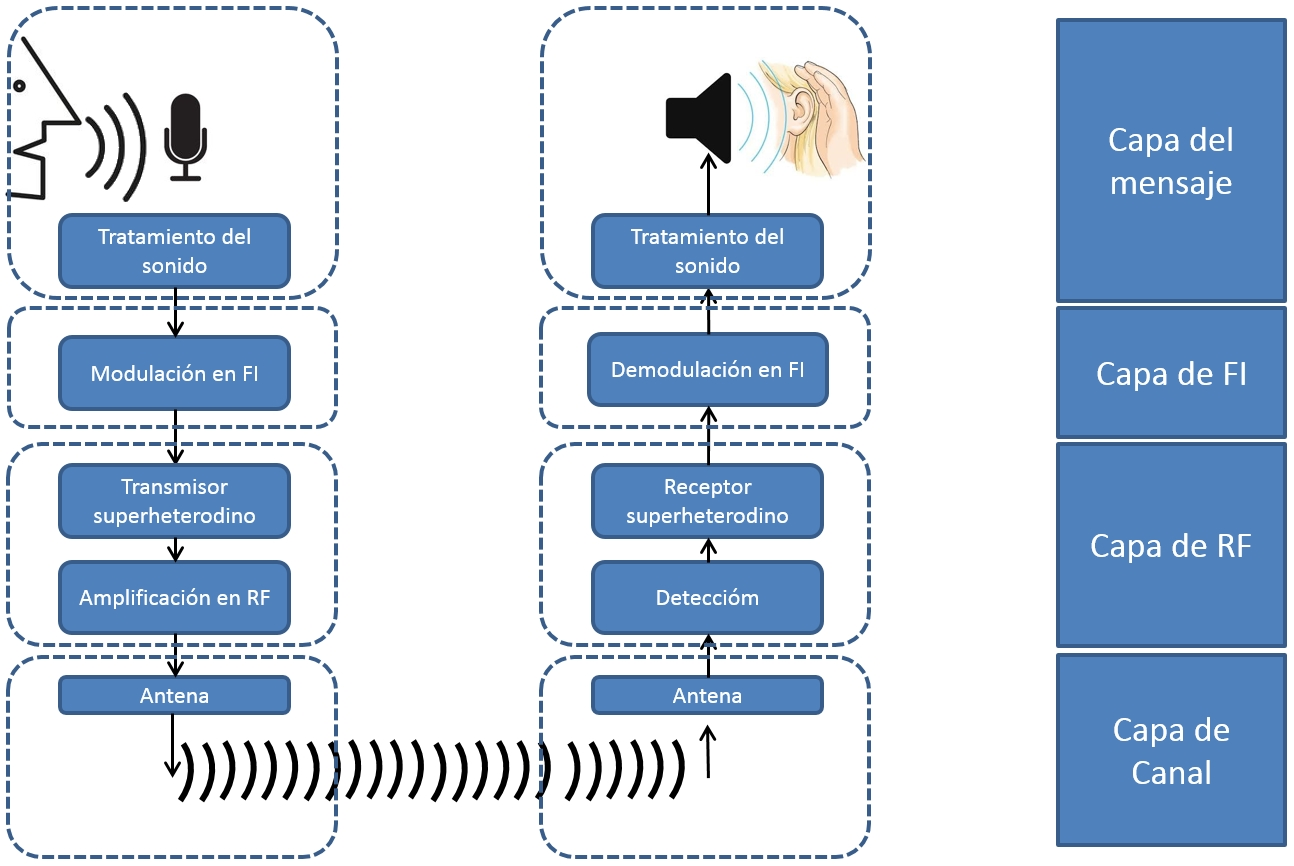
\includegraphics[scale=0.4]{Imagenes/ModeloRadiodifusion}
	\label{fig:ModeloRadiodifusion}
\end{figure}


A diferencia de las comunicaciones punto a punto, en un sistema de radiodifusión se tiene una radio base que emite una señal para que sea sintonizada por cientos o miles de receptores, como es el caso de lo que se conocen como emisoras de radio y de televisión. Como podemos ver, se usan conceptos ya vistos. Las dos capas superiores corresponden al estudio (las oficinas) de una emisora, donde están los equipos que capturan el mensaje de la mejor manera posible, pero también el equipo que realiza la modulación de una señal portadora de frecuencia intermedia que es común para cualquier equipo similar. Por ejemplo, para la radiodifusión AM se ha establecido un valor de frecuencia intermedia igual a 455kHz, mientras que en la de FM es de 10.5 MHz. Las razones para usar una frecuencia intermedia (FI) son las siguientes: \\

\begin{itemize}
	\item  Facilita la separación entre dos tipos de equipos, los que funcionan con baja potencia y baja frecuencia, que pueden usarse en las premisas de la emisora sin temor a causar daños a la salud y los de alta potencia y altas frecuencias, pensados para lograr alcanzar las coberturas necesarias y en las frecuencias necesarias, que deben ser ubicados bajo cuidados especiales, por ejemplo en una torre de comunicación.
    \item  El transmisor superheterodino representa una solución para traducir la señal modulada con FI a una señal modulada con la frecuencia RF. En términos espectrales, consiste en desplazar el espectro de la señal modulada con FI para que quede centrado en la frecuencia $f_c$ como denotaremos en adelante la frecuencia de la portadora o frecuencia RF.
    \item  Igualmente, el receptor superheterodino representa el paso de la señal modulada en la frecuencia RF a la FI
	\item  Gracias a que los valores de FI son estandarizados, es posible combinar el uso de  equipos de diferentes fabricantes para implementar una emisora de radiodifusión.
    \item  Los dispositivos electrónicos usados en cualquiera de las dos etapas se pueden producir a escala a precios bajos ya que tienen funciones limitadas.
\end{itemize}

En la práctica, el modelo de capas de un sistema de radiodifusión puede ser algo más complejo ya que el estudio se localiza usualmente en un lugar poblado, como una ciudad, mientras que los equipos de transmisión, organizados en una radio base, se ubican usualmente en una montaña desde la cual es posible emitir una señal con suficiente potencia para cubrir un gran zona geográfica. Eso significa la necesidad de introducir un sistema adicional de comunicación punto a punto para comunicar el estudio con la radio base. Por ahora no resulta conveniente entrar a revisar un modelo de capas para este caso.\\


%%%%%%%%%%%%%%%%%%%%%%%%%%%%%%%%%%%%%%%%%%%%%%%%%%%%

